\documentclass[11pt]{article}

\usepackage[a4paper,margin=1.5in]{geometry}
\usepackage[strict]{changepage}
% \usepackage[scale=0.92]{tgschola}
% \usepackage{fouriernc}
\usepackage{lmodern}
% \usepackage{libertinus}
\usepackage{inconsolata}
\usepackage[T1]{fontenc}

\usepackage{booktabs, threeparttable, adjustbox, tabularx, longtable}
\usepackage{amsmath, amssymb, amsthm, bbm}
\usepackage{hyperref, achicago}
\usepackage{caption, graphicx}
\usepackage{secdot, sectsty}
\usepackage{pdflscape}
\usepackage{placeins}
\usepackage{xcolor}
\usepackage{titling}

\usepackage[backend=bibtex, style=authortitle, citestyle=authoryear-icomp, maxcitenames=2, url=false]{biblatex}
\addbibresource{Lottery.bib}

\linespread{1}
\urlstyle{tt}

\sectionfont{\centering\normalfont\normalsize\scshape}
\subsectionfont{\centering\normalfont\normalsize\selectfont\itshape}
\subsubsectionfont{\centering\normalfont\normalsize\selectfont\itshape}

\sectiondot{subsection}

\renewcommand{\abstractname}{\vspace{-\baselineskip}}

\renewcommand\thesection{\Roman{section}}
\renewcommand\thesubsection{\thesection.\Alph{subsection}}
\renewcommand\thesubsubsection{\thesubsection.\arabic{subsubsection}}

\newcommand{\specialcell}[2][c]{\begin{tabular}[#1]{@{}c@{}}#2\end{tabular}}
\renewcommand{\today}{\ifcase \month \or January \or February \or March \or April \or May  \or June \or July \or August \or September \or October \or November \or December \fi \number \year}

\begin{document}

\title{\textsc{The Role of Regret in Prize-Linked Savings: Experimental Evidence from Kenya}\protect\footnote{We are grateful to the study participants for generously giving their time. We thank Jonathan Page and Arun Varghese for invaluable research assistance. This study was pre-registered with the AEA RCT registry (AEARCTR-0000893). Files for replication are available at \url{https://github.com/princetonbpl/akiba-lottery-pub}.}}

\author{
	Justin Abraham
		\thanks{Department of Economics. University of California, San Diego. \protect\href{mailto:jabraham@ucsd.edu}{\nolinkurl{jabraham@ucsd.edu}}.},
	Merve Akbas
		\thanks{Department of Economics. Duke University. \protect\href{mailto:merve.akbas@duke.edu}{\nolinkurl{merve.akbas@duke.edu}}.},
	Dan Ariely
		\thanks{Fuqua School of Business. Duke University. \protect\href{mailto:dan@danariely.com}{\nolinkurl{dan@danariely.com}}.}, and
	Chaning Jang
		\thanks{The Busara Center for Behavioral Economics. \protect\href{mailto:chaning.jang@busaracenter.org}{\nolinkurl{chaning.jang@busaracenter.org}}.}
}

\maketitle

	\begin{abstract}

		We conduct a field experiment that randomly assigned 311 informal residents of Nairobi to either a prize-linked savings account (PLS)---a product that incorporate stochastic returns to deposits---against standard, interest-bearing accounts of equivalent expected value. Individuals saving with PLS with feedback made 42\% more deposits on average over the project period than participants who received the fixed incentive. By manipulating the information structure of the PLS treatment, we attribute 20\% of this effect to aversion of regret arising from winning the lottery but not being able to claim the prize. We also present evidence that recent experiences of regret induce greater deposits in the future. We do not observe any effects of the lottery incentive on the amount deposited with PLS or on savings with other products. Lastly, we document limited evidence that use of PLS results in a 15\% increase in gambling activity.

		% On framing: but it's not like regret lotteries are the standard. Instead can employ regret lotteries to boost incentive.

		\medskip \noindent
		JEL Classifications: D14, E21, G11

 	\end{abstract}

\newpage

\section{Introduction}

	% Publication depends on (1) the importance of the question and of the main results; (2) the  clarity,  organization,  and  length  of  the  paper;  and  (3) its degree of novelty in either method or data.

	% Somville structure: introduce default effect, statement of empirical contribution, empirical strategy, hypothesis then preview of results, interpretation of results, contributions/literature

	% Schaner structure: policy motivation, experiment, results preview, mechanism/interpretation, contributions/literature

	The ability to save is one of the most important avenues toward economic development; it provides a means to smooth consumption under incomplete insurance and it makes possible productive investments in the presence of credit constraints. There exists, however, a host of obstacles that prevent poor households from accruing savings to their advantage. There are supply-side limitations to formal finance, such as high initial and transaction costs, that may be prohibitive for the poor. As a result, they often have to resort to methods of saving that can be costly and have limited functionality \parencite{collins_portfolios_2009,karlan_savings_2014,banerjee_economic_2007,schaner_cost_2011}. 

	On the demand side, knowledge gaps, mistrust of financial institutions, and behavioral biases prevent the poor from saving as much as they would like. Less than 20\% of banked adults in Sub-Saharan Africa make more than 2 deposits in a month \parencite{demirguc-kunt_global_2015}. Policies that target costs on the supply side are known to increase account ownership but have been less effective at encouraging usage \parencite{dupas_why_2013,karlan_banking_2016}. Meanwhile, savings products designed to address behavioral barriers have been shown to be extremely cost-effective, especially compared to direct subsidies.\footnote{\textcite{karlan_price_2018} estimate very low interest rate elasticities and limited impacts of easing account ownership requirements. \textcite{schaner_persistent_2018} boost short-run individual savings by USD 1.38 with rates of up to 20\%.} Track-keeping objects \parencite{akbas_how_2016}, SMS reminders \parencite{karlan_getting_2010}, and default contributions \parencite{thaler_save_2004,chetty_active_2014,somville_saving_2018} which address undersaving due to limited attention. Binding commitment devices, in the form of account restrictions \parencite{ashraf_tying_2006} or the application of social pressure \parencite{dupas_why_2013}, can help individuals with time-inconsistent behavior follow through on saving. This literature has demonstrated the importance of product design or \textit{choice architecture} in financial decisionmaking.

	This article examines the potential of prize-linked savings (PLS)--- a savings product that incorporate lottery-like payoffs---in encouraging saving. The key novelty of PLS accounts is that users receive a stochastic payoff in addition to, or in lieu of, interest payments. Common among PLS products is that consumers face no risk of negative returns, at least guaranteeing the full principal amount. PLS have been in use since at least the 17\textsuperscript{th} century and presently exist in various forms around the globe \parencite{murphy_lotteries_2005,kearney_making_2010}. In the United States, PLS accounts are primarily offered at the state level by local credit unions. The American Savings Promotion Act, signed into law in 2014, authorized financial institutions to provide PLS nationwide. Any kind of savings product that allows consumers to enter raffles or earn lottery tickets conditional on deposits may be considered PLS. Products available in Latin America, for instance, offer in-kind prizes. Lottery bonds (like the NS\&I Premium Bonds in the U.K.) are closely related products that provide consumers with the opportunity to redeem bonds for an amount greater than their face value. These products all offer the stochastic component with an eye towards incentivizing further saving.\footnote{It has also been argued that PLS might be advantageous in the Islamic banking sector since lottery winnings can be understood to be in compliance with Sharia law which forbids earning guaranteed interest on assets \parencite{ruth_how_2018}.}

	We conducted a field experiment to analyze the effects of PLS on savings behavior over time. We provided a mobile savings product to 311 informal residents in Nairobi, Kenya and observed account activity over a 60-day period. Using mobile savings allowed us to minimize transactions costs and to collect detailed data on individual transactions. Roughly one-third of our sample was randomly assigned a savings account which matched contributions at 5\%. A second group was assigned an account that yielded stochastic returns equal in expectation to the 5\% match through a daily lottery. Each day, participants received a lottery ticket whose earnings were proportional to amount saved that day instead of a certain match. We compared the match and lottery groups to determine how PLS impacts savings behavior. We find that participants using PLS made 42\% more deposits on average over the project period than participants receiving the matching incentive. This amounts to 5-6 additional days that treated participants made deposits to their savings account. We find no effect of PLS on total amount saved, a finding largely consistent with earlier experimental results. Consequently, we find no evidence that PLS displaced savings from other sources. 

	We also examined the effect of PLS on gambling consumption. While the lottery component could act as a substitute to other forms of gambling, addiction theories of gambling \parencite{becker_theory_1988} suggest complementarities between past and current consumption. Increased access to savings in general could decrease demand for gambling if it is used a means to finance lumpy expenditures in the presence of financial constraints \parencite{herskowitz_gambling_2016}. To answer this question, we estimate effects of PLS on overall gambling by our participants and find that those in the PLS treatment reported higher gambling activity 15 percentage points more than the control group. We do not observe heterogeneous effects on any outcomes by preferences for risk or by an index of problem gambling.

	There are a host of theoretical explanations behind the apparent demand for PLS as opposed to standard savings. Our second objective is to quantify the role of regret aversion \parencite{bell_risk_1983,loomes_regret_1982} as a specific mechanism driving our treatment effects. Regret theory refers to a class of behavioral models that posit that individuals minimize anticipated regret arising from the comparison of prospects against foregone outcomes. In the context of uncertainty, regret aversion has been shown to promote apparently risk averse and risk-seeking behavior  \parencite{zeelenberg_consequences_1996}. 

	To test for regret aversion, we implemented a third treatment wherein participants received the same PLS account with the additional feature that they received a lottery ticket and observed the lottery results only after they had made a deposit that day. That feedback about hypothetical lottery results affects decisions to save is a central prediction of regret aversion. We find that when the resolution of lotteries depends on saving, the effect of PLS on deposits is 20\% smaller than when feedback is always given. In other words, participants assigned to PLS with feedback are motivated to save (and enter the lottery) in anticipation of regret they may feel from having a winning ticket but not being able to claim the prize. Exploiting the longitudinal nature of our data, we also find that recent experiences of regret increase the likelihood of making a deposit in subequent days by 8\%. Together, our evidence points to the importance of regret aversion in demand for PLS.

	This study is one of the first field experiments conducted on PLS in a low-income setting\footnote{\textcite{loibl_testing_2016} conducted a randomized evaluation of IDAs in the U.S. that incorporated a lottery-based savings match. That study found no significant effect of the program relative to guaranteed matching, even when it was bundled with reminder calls and frequent deposit deadlines. They attribute the result to liquidity constraints among their sample, which potentially precluded the benefits of behavioral interventions.}. Much of what we know about the behavioral effects of PLS comes from laboratory studies which provide evidence of a positive effect of stochastic returns on saving. \textcite{atalay_savings_2014} conducted an online portfolio-choice experiment that resulted in participants saving an additional 12 percentage points more with lottery-linked and regular savings than with regular savings alone. Notably, participants who saw an increase in total savings shifted away from lottery expenditures and consumption rather than from regular savings. \textcite{filiz-ozbay_lottery_2015} found participants are more likely to delay payments with lottery-like returns compared to guaranteed interest of equivalent expected value.

	Outside the laboratory, evidence surrounding PLS is as limited\footnote{Lottery-based incentives in other domains, including labor supply \parencite{brune_effect_2015} and health-related behaviors \parencite{kimmel_randomized_2012,bjorkman_nyqvist_using_2015}, are found to have significant effects.}. Our study comes closest to \textcite{dizon_leveraging_2016}, which is a lab experiment conducted with low-income participants in Haiti. The experiment adapts the portfolio allocation task of \textcite{atalay_savings_2014} and found that the introduction of PLS increased gross savings by 22\% financed by a reduction in lottery expenditure and conventional savings. They also find evidence that it is the presence of lottery incentives and not expected returns or the degree of risk that matters for savings. \textcite{gertler_long-term_2017} is the first field experiment studying the long-term effects of PLS in Mexico. They found that bank branches offering PLS saw 41\% more account openings and that these continued to be used five years after the lottery incentives expire. We contribute to this line of research by studying a yet untested feature of PLS (feedback on lottery results) and in so doing we quantify the role of regret aversion as an underlying behavioral mechanism.

	Our experiment also joins a strand of the behavioral literature studying the applicability of regret aversion. \textcite{zeelenberg_consequences_2004} is a cross-sectional study of Dutch lotteries that showed that feedback about winnings in one lottery elicits feelings of regret and that it influences decisions to play. \textcite{barberis_individual_2006} argues that regret aversion is a possible explanation for the reluctance of households to participate in the stock market. \textcite{filiz-ozbay_auctions_2007} finds evidence that regret felt by bidders who lose can explain overbidding in first price auctions. As in this study, they utilize the manipulation of feedback about the winning bid to test for regret aversion. Our study contributes to this literature in examining the implications of regret aversion for household finance and in repeated settings. Namely, we find evidence that regret aversion appears more intense among those who recently experienced regret. A recent paper by \textcite{imas_regret_2016} argues that regret aversion results in an \emph{undervaluation} of lotteries in repeated settings because frequent experiences of regret may dissuade individuals from making risky choices and because feedback provides individuals the opportunity to learn about the incentives. \textcite{strack_too_2019} study a stopping problem when agents are regret averse. They show that decisionmakers a reluctant to stop because they utility depends on the best foregone outcome from the entire history. Regret aversion in repeated settings remain a largely unexplored area of research.

	The remainder of the paper is structured as follows. Section \ref{sec:design} describes our experimental design, Section \ref{sec:est} outlines our estimation strategy, Section \ref{sec:results} presents and discusses our main results, and Section \ref{sec:conclusion} concludes.

		% why people insure and gamble is a longstanding economic puzzle wiwth many explanations coming to fore to explain it
			% friedman savage, machina's paradox
		% can classify theories into three main categories
			% preferences for skewness
			% subjective probabilities
			% specific to developing settings: as a form of saving
		% what are the implications of believing one over the other?
			% what are the behavioral predictions and how do empirical regularities match up?
		% theoretically, this is why PLS are promising

		% why is theory of regret important in the first place? (why did we choose to test it?)
		% what are the prevailing theories of regret?
		% how does this relate to gambling?
		% what are the behavioral predictions and how do empirical regularities match up?

	% How might lotteries induce savings? Preferences for skewed returns are well-documented, so the use of lottery-like structures may play a viable role in incentivizing savings. Models departing from expected utility theory incorporate the overweighting of small probabilities \parencite{kahneman_advances_1992} and attention to salient payoffs \parencite{bordalo_salience_2012} in order to account for seemingly risk-loving behavior among risk-averse individuals. Research on preferences for skewness have produced a litany of potential explanations for this phenomenon.\footnote{This paper does not test against these competing explanations and introduces them as a framework for interpreting results.} One broad strand of the literature understands the overweighting of long-odds as a result of persistent preferences for such gambles. Playing the lottery may provide excitement from taking risks and a chance to win a large payoff \parencite{conlisk_utility_1993}. Similarly, aversion to anticipated regret from foregoing a big prize could drive gambling behavior \parencite{loomes_regret_1982,zeelenberg_consequences_2004}. Credit-constrained households may also rely on lotteries to save for large, indivisible expenditures \parencite{kwang_why_1965,herskowitz_gambling_2016}. Alternatively, preferences for gambling may result from bias in subjective probabilities vis-\`{a}-vis true probabilities. The biased weighting of probabilities implies more fickle gambling behavior that depend on exposure to information and repeated choice \parencite{hertwig_descriptionexperience_2009}.

	% Extensive research has tried to explain the higher demand for lotteries and gambling among people with lower income. One approach allows individuals to use subjective probability weighting to over-weight low probability events, e.g. rank-dependent expected utility theory (Quiggin, 1982); cumulative prospect theory (Tversky and Kahneman, 1992). Another approach, skewness, allows utility to depend upon both absolute and relative wealth so that lotteries offer an opportunity to move up in terms of relative wealth (Shefrin and Statman, 2000). Crossley et al. (2011) suggest that people can use lotteries to convexify their budget sets.

	% Herzkowitz: without savings, gambling is how people can purchase non-divisible durable assets.

	% what is the link to regret aversion? the first point has to do with risk attitudes the second point has to do with violations of independence
	%  The Probability Weighting Function (Drazen Prelec )
	% check lit review in the notes section
	% bilal zia paper on debiasing
	% The Utility Analysis of Choices Involving Risk  friedman savage

\section{Experimental Design} \label{sec:design}

	\subsection{Sampling Frame}

		We conducted our experiment in conjunction with the Busara Center for Behavioral Economics with 311 participants recruited from Nairobi's low-income neighborhoods. Three quarters of our sample reside in Kibera, the city's largest informal settlement. We drew a random sample of participants over 18 years old using SMS and phone calls from the Busara Center's active pool of over 11,000 Nairobi residents. Nearly 60\% of our sample is female with a median age of 28 years. Less than half of the participants in our sample reported that they are employed with only 5\% reported receiving a regular income. The employed in our sample largely work in retail or are students. The median PPP-adjusted monthly income among those employed is USD 77.\footnote{Monetary payouts were in Kenyan shillings (KES). We report USD values calculated at purchasing power parity using a conversion factor for private consumption of 38.15 in 2013. The price level ratio of PPP conversion factor (GDP) to KES market exchange rate for 2011 was 0.444.}

		Approximately 55\% of our sample saves regularly with a majority of savers utilizing rotating savings and credit associations (ROSCA), a type of informal group savings. The average stock of savings among these individuals amount to USD 23. A significant fraction of savers also report using M-Shwari, a mobile service that provides a lockbox account and offers short-term credit.\footnote{The savings product we designed is comparable to M-Shwari in that it also offered commitment savings and a 5\% return on deposits.} Mobile transactions are made with M-Pesa, an SMS-based money system made accessible by the ubiquity of mobile phones in Kenya.

		The surge of mobile phone usage in Kenya has driven the recent popularity of mobile sports betting. SportPesa, one of the most popular mobile gambling services, reports over 800,000 registered users as of 2015 \parencite{kemibaro_sportpesa_2015}. In our sample, 24\% of participants at baseline report that they have some problem with gambling. 11\% of participants report that they gamble at a casino, bet money at racetracks or sporting events, played the sweepstakes, or played cards for money daily or more frequently in the last 12 months.

	\subsection{Data Collection}

		Participants were first invited to the lab at the Busara Center where they completed a computerized questionnaire and behavioral tasks. Experimental sessions included up to 25 participants at a time and were administered in English by research assistants. The following outlines the schedule of tasks during the lab portion of the study:

		\begin{enumerate} \setlength{\itemsep}{1pt}
		\item Coin toss task \parencite{eckel_sex_2002}\footnote{This elicitation method produces interval estimates of the coefficient of relative risk aversion, $\rho$, under the assumption of constant relative risk aversion. We take the midpoint of the upper and lower intervals as point estimates. For participants with $\rho \geq 3.46$ and $\rho \leq 0$, we use boundary values as point estimates.}
		\item Titration task for temporal discounting \parencite{cornsweet_staircase-method_1962}
		\item Willingness-to-pay to play a lottery
		\item Candian Problem Gambling Index \parencite{ferris_canadian_2001}
		\item Internal locus of control \parencite{rotter_generalized_1966}
		\item Demographics questionnaire
		\end{enumerate}

		At the conclusion of the demographics questionnaire, participants received KES 200 for completing the session and an additional KES 50 for arriving on time. Lab sessions took place over five weeks in May and June of 2014. We refer to this period before beginning the savings program as the baseline.

		Following the lab session, participants were enrolled in the 60-day savings program and randomly assigned to one of three incentive schemes: one fixed match and two lottery-based matches. Savings incentives are detailed in Section \ref{sec:treat}. Each participant received KES 20 airtime credit and asked to practice saving using Sambaza. Participants then received business-card sized handouts which described their savings program and bonuses. We provided participants simple instructions for saving and listed the number to our project phone. This was the number through which the savings program operated that also functioned as a help line for participants.

		All participants completed the savings program by August 2014. In September 2014, we called participants and conducted an endline survey that included questions on outside savings, gambling activity, and program feedback. We obtained endline surveys for all but 27 of the 311 participants. We find no evidence that completion of the endline survey correlates with treatment assignment.

		\clearpage

	\subsection{Mobile Savings Product}

		We implemented our 60-day mobile-phone savings program over Safaricom's Sambaza airtime sharing service. Using Sambaza, Safaricom users can send airtime to each other free of charge. Participants saved into our program by sending airtime to a designated project phone that held the airtime in an account for each user.

		Participants received two SMS messages every morning after the first morning of the project period. The first message arrived at 8:00 daily summarizing how much the participant saved the previous day, how much the participant earned through a matching contribution or winnings, and their total balance. An hour later, participants received a beginning-of-day message encouraging them to save that day. Participants were allowed to send in savings at any time but any savings sent in after first message with the lottery results would be counted towards the next day's total. We used a custom-developed administrative system to manage the savings program. This system logged airtime sent to our project phone, maintained an internal ledger of balances, sent automated SMS confirmations after every transaction, and conducted the daily lottery game.

		Participants enrolled in the savings program for two consecutive periods of 30 days starting from the day of a participant's lab session. On a participant's 30th day, a field officer called them and asked if they wished to withdraw any amount of their balance. Participants who requested withdrawals were sent tranfers equal to their plus a withdrawal fee compensation. The product we provided was a ``lockbox'' account where regular withdrawals outside of this opportunity were prohibited.\footnote{This feature is commonplace among informal savings and is increasingly incorporated into savings interventions. \textcite{ashraf_tying_2006} provides evidence that commitment savings increases long-term savings among women who exhibit present-biased time preferences. Commitment savings may also be advantageous when intrahousehold bargaining hinders saving \parencite{banerjee_economic_2007,schaner_cost_2011}.} Transfers were made using the mobile money system M-Pesa to minimize transaction costs. M-Pesa accounts are associated with a SIM card and transactions are made via SMS. Participants could deposit and withdraw money from the account at any of more than 10,000 agents throughout Kenya, including those located in the informal settlements where our participants reside.

		Participants were called and notified a few days before the end of their second 30-day period that the program would be ending soon. After receiving the end-of-day message on their 60th day, participant were unenrolled from the program and were no longer allowed to save. Field officers called participants to confirm final balances and sent M-Pesa transfers equal to total balances net of withdrawals shortly after. Participants paid no explicit fees to participate in our program.

	\subsection{Treatment} \label{sec:treat}

		Participants enrolled in the savings program were randomized into one of three different incentive schemes described below and summarized in Table \ref{tab:treatments}.

		\begin{enumerate} \setlength{\itemsep}{1pt}

			\item \textit{Matching contributions:} Participants in the matching group earned a 5\% matching contribution on any amount that they saved on a particular day. The match was automatically added to the mobile account. The amount of the incentive and the participants' daily balance were reported every morning via SMS. We take this group as our control group.

			\item \textit{Prize-linked savings with feedback:} Every day, participants earned a lottery ticket transmitted via SMS that could win a cash prize in proportion to the amount they saved on the same day.

			A lottery ticket was a random sequence of four numbers between 1 and 9, inclusive. Each morning, our administrative system randomly generated a winning sequence of four numbers. Prizes were awarded according to how well a participant's lottery numbers matched the winning numbers. If the first or second numbers matched, a 10\% match of savings was awarded. If both the first and second numbers matched, a 100\% match of savings was awarded. Finally if all numbers matched, a prize of 200 times the daily savings was awarded. The expected earnings on this lottery ticket were equal to the 5\% match earned in the control group---\textit{i.e.} the expected payoffs were equivalent but by a mean-preserving increase in risk.

			Our system entered winnings into the internal ledger and reported lottery results via SMS the following day. Participants with winning lottery tickets who did not save could not claim the prize but received feedback on their lottery results daily. We henceforth refer to this group as the PLS group. 

			\item \textit{Prize-linked savings without feedback:} This scheme is identical to the Lottery treatment except participants in this third group only received lottery tickets and made aware of their potential winnings if they made a non-zero deposit the previous day. We henceforth refer to this group as the No Feedback group. We leverage the variation of the information regime in this treatment group to test for regret aversion as detailed in Section \ref{sec:mechanisms}.

		\end{enumerate}

		\begin{table}[h!] \centering
			\caption{Summary of treatment conditions} \label{tab:treatments}
			\maxsizebox*{\textwidth}{\textheight}{ \begin{threeparttable} \begin{tabular}{l cc cc cc}
			\toprule
			Treatment & Control Group & PLS (feedback) & PLS (no feedback) \\
			\midrule
			Incentive type & Certain & Stochastic & Stochastic \\
			Expected match rate & 5\% & 5\% & 5\% \\
			View lottery results & N/A & Always & On deposit \\
			\bottomrule \end{tabular}
			\begin{tablenotes}[flushleft] \item \footnotesize \textit{Notes}: A lottery ticket was a random sequence of four numbers between 1 and 9, inclusive. Prizes were awarded according to how well a participant's lottery numbers matched the winning numbers. If the first or second numbers matched, a 10\% match of savings was awarded. If \emph{both} the first and second numbers matched, a 100\% match of savings was awarded. If all numbers matched, a prize of 200 times the daily savings was awarded. \end{tablenotes}
			\end{threeparttable} }
		\end{table}

		\clearpage

\section{Empirical Strategy} \label{sec:est}

	\subsection{Average Treatment Effect}

		We use the following reduced-form specification to estimate the treatment effect of lottery incentives on participant outcomes at the end of the savings period.

		\begin{equation} \label{eq:teffect}
			Y_{i} = \beta_{0} + \beta_{1}\text{NF}_{i} + \beta_{2}\text{PLS}_{i} + \varepsilon_{i}
		\end{equation}

		$Y_{i}$ refers to the outcome variables for individual $i$ measured after the end of the savings program. NF$_i$ indicates assignment to the No Feedback group and PLS$_i$ indicates assignment to the PLS group. The omitted group is the control group. We test $\beta_{1} = 0$ and $\beta_{2} = 0$ to identify the effects of PLS and PLS without feedback relative to the control group. We additionally test $\beta_{2} - \beta_{1} = 0$ for differential effects between the two PLS treatments. Statistical inference is based on heteroskedastic-robust standard errors.

		% To improve precision and to control for potential selection bias, we apply covariate adjustment with a vector of baseline indicators.\footnote{We include as control variables 1. Participant is female, 2. Participant is younger than 30 years old, 3. Participant completed primary school, 4. Participant is married, 5. Participant has at least one child dependant, 6. Participant uses a savings account, and 7. Above median CPGI score.} We obtain the covariate-adjusted treatment effect estimate by estimating Equation \ref{eq:teffect} including the demeaned covariate vector $\mathbf{X}_{i}$ as an additive term and as an interaction with the treatment indicator.

		% \begin{equation} \begin{split} \label{eq:controls}
		% 	Y_{i} = & \beta_{0} + \beta_{1}\text{NF}_{i} + \beta_{2}\text{PLS}_{i} + \mathbf{X}'_i \gamma_{0} \\
		% 			& + \text{NF}_{i} \mathbf{X}'_i \gamma_{1} + \text{PLS}_{i} \mathbf{X}'_i \gamma_{2} + \varepsilon_{i}
		% \end{split} \end{equation}

		% The set of indicators partitions our sample so that our estimate remains unbiased for the average treatment effect \parencite{lin_agnostic_2013}. As in Equation \ref{eq:teffect}, we test $\beta_{1} = 0$ and $\beta_{2} = 0$ to identify the effects of the PLS with and without feedback relative to the matching group and test $\beta_{2} - \beta_{1} = 0$ for differential effects between the two PLS treatments. Standard errors are clustered at the individual level. Equation \ref{eq:teffect} is our preferred specification and report results with covariate adjustment for robustness.

		We might expect that the errors of each outcome variable are correlated. Instead of estimating these equations separately, we estimate the system of seemingly unrelated regressions (SUR) to improve the precision of the coefficient estimates \parencite{zellner_efficient_1962}. SUR estimation is equivalent to OLS when the error terms are in fact uncorrelated between regressions or when each equation contains the same set of regressors. We perform joint estimation over outcome groups for Equation \ref{eq:teffect}.\footnote{Grouping of dependant variables was specified in a pre-analysis plan.}

		We control for the family-wise error rate (FWER) to correct for multiple inference. We compute adjusted $p$-values within categories of outcome variables using the free step-down resampling method \parencite{westfall_resampling-based_1993,anderson_multiple_2008}. This approach sets the size of the test to exactly the desired crticial value. We apply this correction over outcome variables in each family and separately for each hypothesis test. For each variable, we apply the procedure with 10,000 iterations and report both unadjusted and adjusted $p$-values.

	% \subsection{Minimum Detectable Effect Sizes}

	% 	To determine whether our null findings identify the absence of a true effect or signify a lack of statistical power, we report the minimum detectable effect size (MDE) for each outcome.

	% 	\begin{equation}
	% 		\mathrm{MDE}_{\hat \beta} = (t_{1-\kappa} + t_{\alpha/2}) \times \mathrm{SE}(\hat \beta)
	% 	\label{eq:mde} \end{equation}

	% 	This metric is the smallest effect that would have been detectable given our current sample size. Thus, a MDE greater than our estimated treatment effect suggests that null results are due to a lack of statistical power. We calculate MDEs \textit{ex post} with $\alpha = 0.05$ and 0.80 power for both No Feedback and PLS treatment effects.

	\subsection{Heterogeneous Treatment Effects}

		We analyze the extent to which the savings program produced heterogeneous treatment effects with the following specification.\footnote{$\beta$ here denotes a different parameter than those in the previous regressions.}

		\begin{equation} \begin{split}
		Y_{i} = & \beta_{0} + \beta_{1}\text{NF}_{i} + \beta_{2}\text{PLS}_{i} + \delta_{0}x_{i} \\
					& + \delta_{1}(\text{NF}_{i} \times x_{i}) + \delta_{2}(\text{PLS}_{i} \times x_{i}) + \varepsilon_{i}
		\end{split} \label{eq:heteffect} \end{equation}

		$x_{i}$ is the binary dimension of heterogeneity measured before treatment assignment. $\delta_{1}$ and $\delta_{2}$ respectively identify the heterogeneous treatment effects of the two PLS products relative to individuals whose $x_{i} = 0$. We conduct inference with heteroskedstic-robust standard errors. We report estimates with the following baseline variables as $x_{i}$: an indicator for prior usage of a savings account, an indicator for scoring above the median in the CPGI scale, an indicator for being classified as risk averse in the coin toss task, and an indicator for having an above median average indifference point as measured in the titration task.\footnote{We report heterogeneous treatment effects for a wider set of baseline variables in an online appendix.}

	% \subsection{Time-Varying Treatment Effects}
	%
	% 	Using detailed daily transaction data, we can estimate treatment effects of PLS conditional on the time elapsed since the start of the savings program. We estimate a model that interacts the treatment indicators with a linear time trend.
	%
	% 	\begin{equation} \begin{split}
	% 	Y_{i,t} = & \beta_{0} + \beta_{1}\text{NF}_{i} + \beta_{2}\text{PLS}_{i} + \lambda_{0}t \\
	% 				& + \lambda_{1}(\text{NF}_{i} \times t) + \lambda_{2}(\text{PLS}_{i} \times t) + \varepsilon_{i}
	% 	\end{split} \label{eq:timelinear} \end{equation}
	%
	% 	In this equation, $t$ is the number of days since the start of the savings program and $Y_{i,t}$ denotes whether participant $i$ made a deposit at period $t$. We also estimate this equation for $Y_{i,t}$ as the amount deposited in period $t$. $\lambda_1$ is the marginal effect of the lottery incentive on $Y_{i,t}$ with respect to days elapsed. $\lambda_2$ is the marginal effect of lottery with feedback. We test the hypotheses $\lambda_1 = 0$ and $\lambda_2 = 0$---that the effects of PLS are constant as a function of time. Standard errors are clustered at the individual level.
	%
	% 	Using detailed daily transaction data, we can estimate treatment effects of PLS conditional on the time elapsed since the start of the savings program. We estimate day-specific effects with the following specification.
	%
	% 	\begin{equation} \begin{split}
	% 	Y_{i,t} = & \beta_{0} + \beta_{1}\text{NF}_{i} + \beta_{2}\text{PLS}_{i} \\
	% 				& + \sum_{t=2}^{60} \bigg [ \zeta_{t} \tau_{t} + \eta_{t}(\text{NF}_{i} \times \tau_{t}) + \theta_{t}(\text{PLS}_{i} \times \tau_{t}) \bigg ] + u_{i, t}
	% 	\end{split} \label{eq:timedummy} \end{equation}
	%
	% 	$Y_{i, t}$ is the outcome for individual $i$ at period $t$, NF$_i$ indicates assignment to the Lottery group, and PLS$_i$ indicates assignment to the PLS group. $\tau_t$ is an indicator taking the value 1 in period $t$. The omitted group is the control group at $t=1$. We can interpret the value of $\beta_1 + \eta_t$ and $\beta_2 + \theta_t$ as the effects of Lottery and PLS, respectively, at period $t$. We test the null hypothesis of no time-varying treatment effects with a joint tests of $\beta_1 + \eta_t = 0$ and $\beta_2 + \theta_t = 0$, respectively, for $t = 2, \ldots, 60$. Standard errors are clustered at the individual level.

\section{Results} \label{sec:results}

	By the end of the project, the median participant in the control group contributed USD 3.86 to the mobile savings account over 8 deposits. The total saved by the control group amounts to less than 5\% of the median monthly income (USD 77.24) and 17\% of the median monthly savings (USD 22.91). 13\% of the control group did not use their accounts at all. Despite the relatively high 5\% rate of return on deposits, minimal saving is consistent with estimates of low interest rate elasticities \parencite{karlan_price_2018}. Table \ref{tab:tab-lottery} compares the lottery results with the expected probabilities of each type of lottery match. Table \ref{tab:sum-ysumall} reports summary statistics and tests for balance across treatment groups of several pre-treatment characteristics. We find no overall imbalance based on a test of joint significance across all observables.\footnote{We account for the correlation of treatment to usage of a savings account in Section \ref{sec:est}.}

	\begin{table}[htbp]\centering \def\sym#1{\ifmmode^{#1}\else\(^{#1}\)\fi} \caption{Expected and observed lottery results} \label{tab:tab-lottery} \maxsizebox*{\paperwidth}{\paperheight}{ \begin{threeparttable} \begin{tabular}{l*{3}{c}} \toprule
                    &        Freq.&         Pct. observed&      Pct. expected\\
\midrule
No match                   &        7065&       81.49&       62.43\\
One match                   &        1518&       17.51&       22.22\\
Two matches                   &          86&        0.99&       1.23\\
Complete match                   &           1&        0.01&      0.00\\
\bottomrule \end{tabular} \begin{tablenotes}[flushleft] \footnotesize \item \emph{Notes:} The first column tabulates the frequency of observed lottery ticket matches. The second and third columns report the observed and expected probabilities, respectively, of each type of lottery match. A lottery ticket was a random sequence of four numbers between 1 and 9, inclusive. Prizes were awarded according to how well a participant's lottery numbers matched the winning numbers. If the first or second numbers matched, a 10\% match of savings was awarded. If \emph{both} the first and second numbers matched, a 100\% match of savings was awarded. Finally if all numbers matched, a prize of 200 times the daily savings was awarded. \end{tablenotes} \end{threeparttable} } \end{table}


	\begin{table}[h]\centering \def\sym#1{\ifmmode^{#1}\else\(^{#1}\)\fi} \caption{Baseline balance by treatment group} \label{tab:sum-ysumall} \maxsizebox*{\textwidth}{\textheight}{ \begin{threeparttable} \begin{tabular}{l*{5}{c}} \toprule
          &\multicolumn{1}{c}{(1)}&\multicolumn{1}{c}{(2)}&\multicolumn{1}{c}{(3)}&\multicolumn{1}{c}{(4)}&\multicolumn{1}{c}{(5)}\\
          &\multicolumn{1}{c}{\specialcell{No Feedback -\\Control}}&\multicolumn{1}{c}{\specialcell{PLS -\\Control}}&\multicolumn{1}{c}{\specialcell{No Feedback -\\PLS}}&\multicolumn{1}{c}{\specialcell{Control mean\\(SD)}}&\multicolumn{1}{c}{Obs.}\\
\midrule
Female    &     0.07&     0.10&     0.03&     0.52&      311\\
          &   (0.07)&   (0.07)&   (0.07)&   (0.50)&         \\
Age       &     0.78&     0.72&    -0.05&    30.75&      311\\
          &   (1.39)&   (1.34)&   (1.35)&   (9.83)&         \\
Completed std. 8&    -0.02&    -0.02&     0.00&     0.99&      311\\
          &   (0.02)&   (0.02)&   (0.02)&   (0.10)&         \\
Married/co-habitating&     0.10&     0.09&    -0.01&     0.42&      311\\
          &   (0.07)&   (0.07)&   (0.07)&   (0.50)&         \\
No. of children&     0.23&     0.24&     0.01&     1.75&      311\\
          &   (0.24)&   (0.25)&   (0.25)&   (1.70)&         \\
Currently saves&     0.05&    -0.10&    -0.15&     0.56&      311\\
          &   (0.07)&   (0.07)&   (0.07)&   (0.50)&         \\
Total savings last month&   -17.81&    -7.04&    10.77&    58.82&      311\\
          &  (11.88)&  (12.55)&   (9.23)& (106.26)&         \\
Monthly income&    -3.68&    -0.59&     3.09&   112.05&      311\\
          &  (17.63)&  (16.85)&  (15.46)& (137.13)&         \\
Employment status&     0.05&    -0.03&    -0.08&     0.50&      311\\
          &   (0.07)&   (0.07)&   (0.07)&   (0.50)&         \\
Coefficient of relative risk aversion&     0.08&    -0.03&    -0.12&     1.16&      311\\
          &   (0.18)&   (0.17)&   (0.18)&   (1.27)&         \\
Locus of control&     0.48&    -0.83&    -1.31&    69.81&      311\\
          &   (1.40)&   (1.46)&   (1.37)&  (10.78)&         \\
Standardized CPGI&    -0.11&    -0.22&    -0.11&    -0.00&      311\\
          &   (0.13)&   (0.12)&   (0.12)&   (1.00)&         \\
Exp. discount factor&    -0.05&    -0.01&     0.04&     0.33&      311\\
          &   (0.03)&   (0.03)&   (0.03)&   (0.20)&         \\
\midrule Joint test \emph{p}-value&     0.44&     0.72&     0.42&         &         \\
\bottomrule \end{tabular} \begin{tablenotes}[flushleft] \footnotesize \item \emph{Notes:} The first three columns report the difference of means across treatment groups with standard errors in parentheses. Column 4 reports the mean of the control group with SD in parentheses. The bottom row reports the \(p\)-value of a joint test of significance for each hypothesis. \end{tablenotes} \end{threeparttable} } \end{table}

% File produced by sum-treat.do with /Users/justin/Repos/akiba-lottery-pub/data/clean/akiba_wide.dta on 15:49:29 12 Aug 2020 by user justin on Stata 13.1 with seed X53d8cd0fc43f462544a474abacbdd93d00044a8f

	\subsection{PLS Increases Deposit Frequency}

		We find that participants in the PLS group made between 5-6 more deposit transactions ($\hat \beta = 5.71, p < 0.05$) over the entire project period compared to those receiving the match incentive. Column 2 of Table \ref{tab:reg-fwermobile} reports a moderately sized effect of 0.38 SD over the average frequency of deposits in the control group. This result is further robust to the inclusion of control variables and significant at the 10\% level with FWER adjusted $p$-values. These effects exhibit no heterogeneity across prior savings usage, problem gambling, risk attitudes, and temporal discounting (Tables \ref{tab:het-save_dosave_0}- \ref{tab:het-gam_mediancpgi_z_0}). Participants in the PLS treatment had an additional 5 days on average that they chose to make at least one deposit relative to the control ($\hat \beta = 4.94, p < 0.05$). This suggests that the effect on the frequency of deposits occurs on the daily extensive margin; it is not driven by participants depositing more often within a day. This result is robust to covariate adjustment and is significant at the 10\% level after FWER corrections.

		\begin{table}[ht]\centering \def\sym#1{\ifmmode^{#1}\else\(^{#1}\)\fi} \caption{Treatment effects -- Mobile savings} \label{tab:reg-fwermobile} \maxsizebox*{\textwidth}{\textheight}{ \begin{threeparttable} \begin{tabular}{l*{5}{c}} \toprule
          &\multicolumn{3}{c}{Effect estimates}&\multicolumn{2}{c}{Sample}\\\cmidrule(lr){2-4}\cmidrule(lr){5-6}
          &\multicolumn{1}{c}{(1)}&\multicolumn{1}{c}{(2)}&\multicolumn{1}{c}{(3)}&\multicolumn{1}{c}{(4)}&\multicolumn{1}{c}{(5)}\\
          &\multicolumn{1}{c}{Lottery}&\multicolumn{1}{c}{Regret}&\multicolumn{1}{c}{\specialcell{Regret-\\Lottery}}&\multicolumn{1}{c}{\specialcell{Control Mean\\(SD)}}&\multicolumn{1}{c}{Obs.}\\
\midrule
Total no. of deposits&4.59$^{*}$&5.71$^{**}$&     1.13&    13.66&      311\\
          &   (2.52)&   (2.45)&   (2.84)&  (15.08)&         \\
          &   [0.20]&[0.06]$^{*}$&   [0.89]&         &         \\
No. of days saved&3.93$^{*}$&4.94$^{**}$&     1.01&    11.78&      311\\
          &   (2.05)&   (2.08)&   (2.32)&  (12.93)&         \\
          &   [0.17]&[0.06]$^{*}$&   [0.89]&         &         \\
Total deposit amount&    -0.79&    -1.60&    -0.81&    14.87&      311\\
          &   (3.34)&   (2.91)&   (2.88)&  (24.48)&         \\
          &   [0.84]&   [0.59]&   [0.89]&         &         \\
Total withdrawal amount&     0.53&1.63$^{**}$&     1.10&     1.07&      311\\
          &   (0.94)&   (0.74)&   (1.02)&   (4.53)&         \\
          &   [0.84]&[0.06]$^{*}$&   [0.61]&         &         \\
\bottomrule \end{tabular} \begin{tablenotes}[flushleft] \footnotesize \item \emph{Notes:} Columns 1--3 report OLS estimates of the treatment effect. Standard errors are in parentheses and FWER adjusted \(p\)-values are in brackets. Observations are at the individual level. * denotes significance at 10 pct., ** at 5 pct., and *** at 1 pct. level. Stars on the coefficient estimates reflect unadjusted \(p\)-values. \end{tablenotes} \end{threeparttable} } \end{table}

% File produced by reg-fwer.do with /n/homeserver2/user2a/justinra/repos/akiba-lottery-pub/data/clean/akiba_wide.dta on 02:49:49 21 Feb 2018 by user justinra on Stata 13.1 with seed X71d1d353b37e281e006fa26738e26f4500044a1c

		Panel A of Figure \ref{fig:line-cumdeposits} traces the cumulative path of deposits made over the duration of the project. The average number of deposits for the PLS group are greater than for the control group over all periods, though we are only able to statistically distinguish cumulative values at the end of the 60-day period.

		\begin{figure}[ht]
			\caption{Number of deposits and amount deposited over project period}
			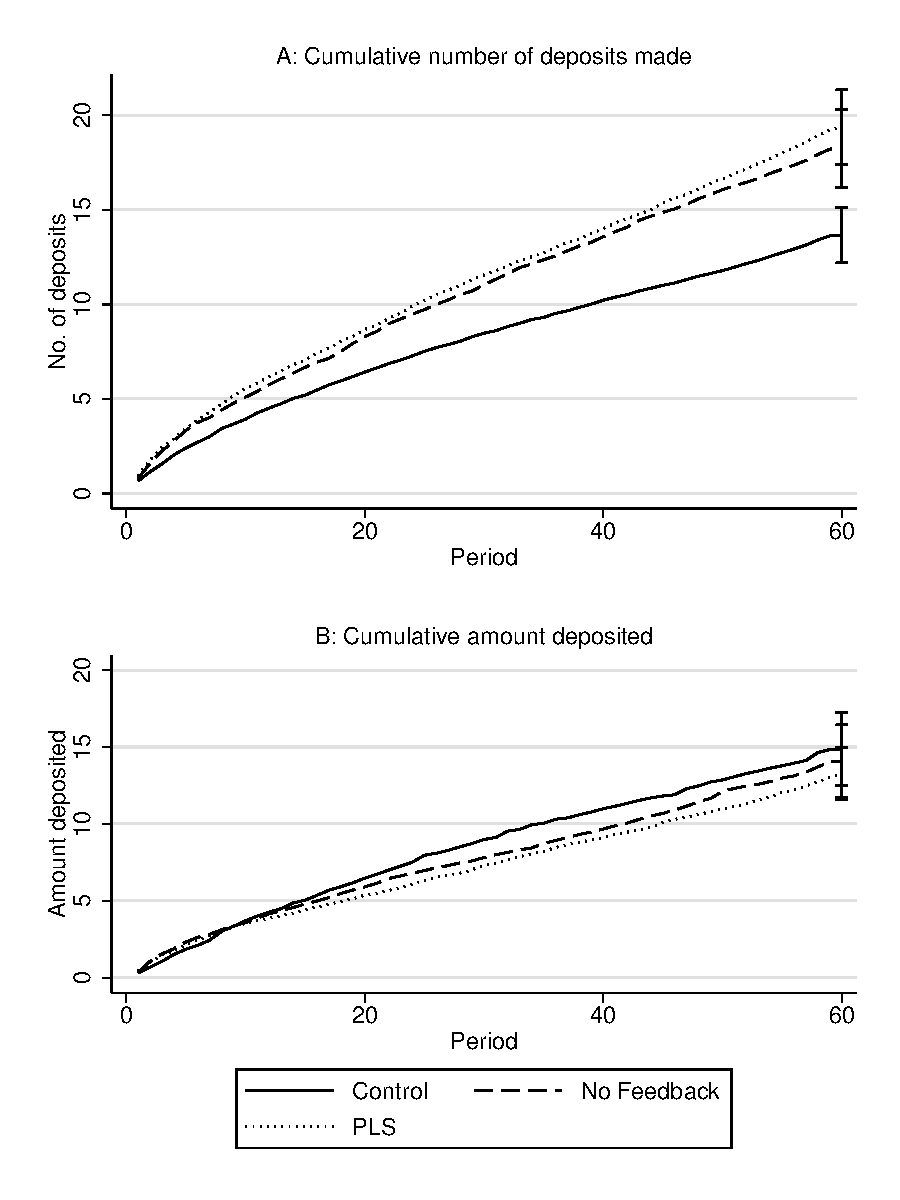
\includegraphics[height=0.85\textheight]{../../figures/line-cumdeposits.pdf}
			\label{fig:line-cumdeposits}
			\caption*{\footnotesize \emph{Notes:} Panel A plots the cumulative number of deposits made by the average participant over the 60-day savings period by treatment assignment. Panel B plots the cumulative amount deposited by the average participant. Error bars for totals by the end of the project are within one standard error of the group means.}
		\end{figure}

		\clearpage

		While effects on number of deposits are considerable, we find no effect of either PLS treatment on total amount deposited over the project period. Panel B of Figure \ref{fig:line-cumdeposits} plots the cumulative deposit amounts, averaged by treatment group, over the 60-day period. We cannot distinguish total deposit amounts between any of the three incentive schemes. Participants in the PLS group withdrew a larger amount relative to the control on average ($\hat \beta = 1.63, p < 0.05$) but we are unable to detect statistically significant differences in the final balance across treatment groups. In fact, account balances at the end of the trial are highest among the control group (mean = $14.13$, std. dev. = $23.11$). More frequent deposits without a corresponding increase in savings and larger withdrawals by PLS users suggest that they may be using their deposits to finance lottery plays and not to build a stock of savings.

		Our results are consistent with a general finding among earlier field experiments on lottery-based incentives that behavioral responses occur on the extensive, but not intensive, margin. \textcite{brune_effect_2015} test a stochastic incentive in Malawi wherein tea harvesters entered a lottery conditional on attendance and could increase their probability of a prize according to their output. That study found significant improvements in workplace attendance, allowing workers to enter the lottery, but without changes in output. \textcite{loibl_testing_2016}, examined features of the Individual Development Account program in the U.S. and found no effect of PLS over certain returns of equal expected value. A recent experiment by \textcite{gertler_long-term_2017} randomized the provision of PLS across banks in Mexico and observed a 43\% increase in the number of account openings in the month the lotteries were in effect but without affecting balances.\footnote{\textcite{gertler_long-term_2017} observes effects on account openings but not on transactions compared to the control group. Our study opened accounts for all participants in the sample.}

		Other experimental results, which \emph{do} find effects on amount saved, are to some degree at odds with our own. \textcite{atalay_savings_2014} conducted an online portfolio-choice experiment in the U.S. that resulted in subjects saving an additional 12 percentage points more with prize-linked and regular savings than with regular savings alone. \textcite{dizon_leveraging_2016} replicate this design in a field experiment conducted in Haiti and identify a 22\% increase in savings.\footnote{\textcite{dizon_leveraging_2016} emphasize that savings responded to the presence of the stochastic incentive rather than its degree of risk or the expected returns.} In an experiment with undergraduates, \textcite{filiz-ozbay_lottery_2015} found that subjects are willing to accept a lower rate of return to delay a payment when the return is stochastic than when it is deterministic. The experimental design of these three studies differed from this one in two respects. First, subjects in those lab studies were supplied with an endowment with which to make portfolio allocations. With a median monthly income of USD 77, households in our study may be too liquidity constrained to sustain a larger balance with PLS\footnote{The presence of liquidity constraints is also the explanation offered in \textcite{loibl_testing_2016} to rationalize a lack of an effect for their PLS product in the US.}. Baseline correlations suggest that monthly income is predictive of savings in the mobile product, though we do not observe heterogeneity of the treatment effect conditional on income. Second, our sample already had access to a number of competing savings products, both formal and informal, which could have dampened demand for PLS savings. To be sure, this discussion does not preclude other factors which could affect the external validity of the results presented here.

		% Dizon does not give feedback, Filiz-Ozbay does not, Brune no, Atalay no, Nyqvist no, Loibl no. So regret aversion can't actually explain prior results. Furthermore, it cannot be a mechanism behind those. The only thing we can say is that it could be used to encourage more saving.

		% Adrian's point about what we should expect people to do at the end of the savings period (put everything and leave), what happens during withdrawals, what does it mean for people to increase deposits but not savings, what the estimand is if preferences aren't stable.

		% In general, what should we expect as we get closer to a date of withdrawal? That savings should be high because discounting isn't as intense. This is not the case. Figure out what's going on.

	\subsection{The Role of Regret Aversion} \label{sec:mechanisms}

		That potential savers respond to PLS by making more frequent deposits without a corresponding increase in balance can be partially rationalized as the subdivision of lotteries to reduce risk \parencite{samuelson_risk_1963}. Under this hypothesis, risk averse individuals will subdivide bets over a greater number of gambles so that the risk of a low return is minimized. Since PLS offers returns equivalent in expectation to the matching incentive, we would expect risk averse individuals to save no more with PLS, but merely spread out deposits, than with the standard account. Yet another explanation for our findings is the ``entertainment'' utility hypothesis of gambling \parencite{conlisk_utility_1993}. That is, consumers will behave in ways that enable them to make gambles because they derive consumption utility from simply playing and irrespective of potential earnings. Under this hypothesis, an increase in the number of deposits in the treatment group is expected if merely making a deposit on a certain day qualifies participants to play the lottery for that day. Recall that participants had almost five more active days---and thus play the lottery five more times---than the control group. Unsurprisingly, participants are not making more deposits \textit{within} days since this does not affect lottery eligibility. For these reasons we expect the PLS to induce more deposits without a corresponding increase in amount saved.

		Our study was designed to investigate the role of regret aversion as a specific mechanism explaining demand for PLS. Regret theory is a class of behavioral models that incorporate an individual's aversion to feelings of regret---an emotional response to foregone opportunities due to action or inaction. \textcite{bell_risk_1983} and \textcite{loomes_regret_1982} were one of the first to formalize this as a complication to expected utility theory. Where expected utility depends only on final outcomes, (dis)utility from regret (rejoicing) depends on the difference between the realized outcome and the best foregone outcome. Hence, theories of regret are action-based rather than purely outcome-based. Regret theory further posits that individuals can anticipate the psychological consequences of the decisions and therefore take them into account ex ante. These class of theories received attention due to their ability to rationalize behavioral deviations from expected utility theory (e.g. the common ratio and common consequences effects).

		\textcite{zeelenberg_consequences_1996} demonstrates how the minimization of anticipated regret can rationalize risk-seeking behavior among risk-averse individuals in situations of \textit{asymmetric feedback}. This describes, for example, choices between a lottery and a certain outcome where choosing the lottery leads to its resolution whereas choosing certainty typically does not involve a resolution of the lottery. Since regret derives from a comparison of foregone outcomes, choosing the lottery and receiving feedback involves the possibility of regret while choosing certainty does not. A regret-minimizing individual would thus find certainty favorable beyond that implied by her risk preferences. Conversely, providing feedback on the lottery regardless of choice (a situation of \emph{symmetric feedback}), removes the anticipation of regret associated with certainty. That feedback influences the anticipation of regret in this way has received empirical support in other applications \textcite{somasundaram_regret_2017,filiz-ozbay_auctions_2007,zeelenberg_consequences_2004}.

		We test for the effect of lottery feedback in our own experiment as a way of quantifying the contribution of regret aversion in the demand for PLS. Recall that in the PLS treatment, the lottery involves no possibility of losses and that lotteries are resolved regardless of saving. Therefore, regret manifests when individuals choose not to save but learn about foregone winnings from the lottery. Regret-minimization predicts that individuals on the margin make deposits in avoidance of this anticipated regret. We compare behavior with an alternate PLS treatment (the No Feedback group) which provided a day's lottery results if and only if the individual made a deposit on that day. Participants in this condition anticipate that choosing not to save involves no regret since they can remain unaware of their foregone lottery earnings. As a result, regret theory predicts greater deposits with feedback than without.\footnote{See Section \ref{sec:model} for a formalization of this argument.} 

		Column 1 of Table \ref{tab:reg-fwermobile} shows that the effect of No Feedback on the number of deposits are positive but smaller in magnitude to the effect of PLS and are not significant at the 5\% level ($\hat \beta = 4.59, p < 0.10$). Column 3 reports on the difference between the PLS and No Feedback conditions, which we do not find statistically significant. The effect of No Feedback on number of days saved follows a similar pattern ($\hat \beta = 3.93, p < 0.10$) compared to PLS with feedback. Our estimates imply that approximately 20\% of the PLS treatment effect can be attributed to regret aversion.

	\subsection{Does Experienced Regret Affect Savings?}

		% motivate this better

		In the theory of regret outlined in the previous section, the anticipation of regret determines ex ante choice. That model makes no predictions regarding the role of recently experienced regret in individual choice. If participants feel the sting of foregone lottery winnings from yesterday, are they more likely to act on their regret aversion today?

		We can leverage the panel structure of our data and the randomness of the lottery results to estimate the effect of recently experienced regret on deposits. If participants are saving in response to experienced regret of foregoing the prize, we expect to see an independent effect of winning the lottery among non-savers on the decision to save in the PLS group. Let $Y_{i,t}$ denote having made a deposit by participant $i$ in period $t$. $\text{Win}_{i,t-1}$ is an indicator for having a winning lottery ticket from the previous day announced in period $t$. We estimate the following equation conditional on assignment to the PLS group and not having saved one period prior.

		\begin{equation} \begin{split}
		Y_{i,t} = & \pi \text{Win}_{i,t-1} + \omega_{t} + u_{i,t}
		\end{split} \label{eq:regret} \end{equation}

		$\pi$ is the additional effect from winning but not being able to claim the prize. $\omega_{t}$ is a period-specific fixed effect. We test the null hypothesis of $\pi = 0$.

		\begin{table}[ht]\centering \def\sym#1{\ifmmode^{#1}\else\(^{#1}\)\fi} \caption{Regression of deposits on lottery results} \label{tab:reg-regretaversion} \maxsizebox*{\textwidth}{\textheight}{ \begin{threeparttable} \begin{tabular}{l*{2}{c}} \toprule
                &\multicolumn{1}{c}{Made a deposit}\\
\midrule
Winning ticket  &     0.02\sym{**} \\
                &   (0.01)         \\
\midrule
Adjusted \(R^{2}\)&    0.081         \\
Control mean    &     0.20         \\
Daily PLS effect&                  \\
Observations    &     4473         \\
\bottomrule \end{tabular} \begin{tablenotes}[flushleft] \footnotesize \item \emph{Notes:} This table reports on a regression of having saved at period \(t\) on winning the lottery at \(t\) conditional on being in the PLS group and not having saved at \(t-1\). The unit of observation is individual-by-period. The regression includes period fixed effects. Standard errors are in parentheses and clustered at the individual level. * denotes significance at 10 pct., ** at 5 pct., and *** at 1 pct. level. \end{tablenotes} \end{threeparttable} } \end{table}

% File produced by akiba-estimate.do with /Users/justin/Repos/akiba-lottery-pub/data/clean/akiba_long.dta on 11:52:17 25 Oct 2020 by user justin on Stata 13.1 with seed Xd950c82044e7d5a124b5a3e57a7d26c000042a30

		Table \ref{tab:reg-regretaversion} shows that the treatment effect is 2 percentage points ($p<0.05$) higher after learning about a winning ticket than learning about a losing one. With an average daily effect of 0.08 of PLS, this account for a fourth of the group treatment effect. Additional evidence comes from Figure \ref{fig:hist-deposits}, which plots the distribution of deposits over time and shows timing suggestive of regret aversion. Nearly all deposits made in the PLS group ocurred within an hour of announcing the lottery results from the previous day. We observe no similar pattern in the No Feedback and control groups. Together, the evidence suggests that recently experienced regret from foregone earnings improves the likelihood of entering the lottery in subsequent rounds.

		\begin{figure}[ht]
		\centering
		\caption{Timing of deposits}
		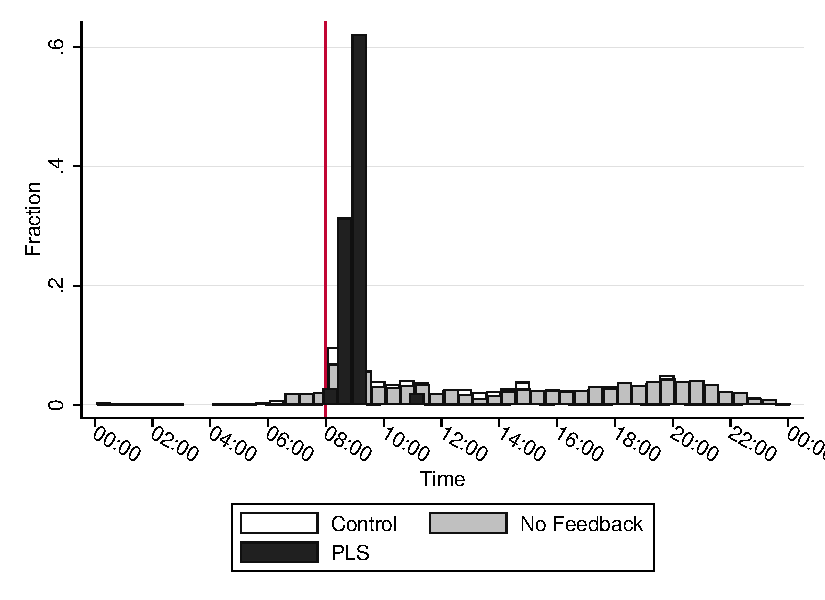
\includegraphics[width=\textwidth]{../../figures/hist-deposits.pdf}
		\label{fig:hist-deposits}
		\caption*{\footnotesize \emph{Notes:} This figure plots the empirical distribution of timing of all deposits over the project period. Each bin spans 30 minutes with a height equal to the fraction of all deposits within each treatment group. A vertical line marks 8:00, when participants received the first SMS that summarized how much the participant saved the previous day, how much the participant earned through a matching contribution or winnings, and their total balance. An hour later, participants received a second SMS encouraging them to save that day. Participants in PLS received a new lottery ticket with the second message.}
		\end{figure}

		\clearpage

	% \subsection{Effect on Deposits Persists Over Time}
	
	% 	The preceding results provide evidence that PLS with feedback compels individuals to make more frequent deposits.

	% Key result: the effect is largest at the outset but converges to 0. But We additionally find no statistically significant heterogeneity by interacting the treatment effect with period indicators.

	% Interpretation: de-biasing literature by Erev et al. regret aversion in repeated settings by Imas et al.

		% we do not find evidence that this decreases (except after the first few days)

		% this has been documented in the lab with small stakes and repeated decisions. erev demonstrates that people who take median 15 (weber 2007 17) with replacement are less likely to overweight rare events. also erev speculates that this is through experience with the rare event and demonstrates it.
		% alternatively, overweighting of recent evidence. does winning affect decision to play in this study?
		% can subjective bias be decreasing over time? (zia paper)
		% brune paper on time dependence
		% which mechanisms are being activated? debiasing, overweighting of recent evidence

		% \begin{table}[ht]\centering \def\sym#1{\ifmmode^{#1}\else\(^{#1}\)\fi} \caption{Time-varying treatment effects on deposits} \label{tab:reg-timedummy} \maxsizebox*{\textwidth}{\textheight}{ \begin{threeparttable} \begin{tabular}{l*{2}{c}} \toprule
                &\multicolumn{1}{c}{Made a deposit}\\
\midrule
Lottery         &     0.10         \\
                &   (0.07)         \\
Regret          &     0.12\sym{*}  \\
                &   (0.07)         \\
Constant        &     0.60\sym{***}\\
                &   (0.05)         \\
\midrule
Adjusted \(R^{2}\)&    0.049         \\
Lottery joint \(p\)-value&     0.02         \\
Regret joint \(p\)-value&     0.01         \\
Observations    &    18660         \\
\bottomrule \end{tabular} \begin{tablenotes}[flushleft] \footnotesize \item \emph{Notes:} This table reports a regression of having saved at period \(t\) on treatment indicators interacted with period indicator variables. The unit of observation is individual-by-period. Standard errors are in parentheses and clustered at the individual level. * denotes significance at 10 pct., ** at 5 pct., and *** at 1 pct. level. \end{tablenotes} \end{threeparttable} } \end{table}

% File produced by akiba-estimate.do with /Users/justin/Repos/akiba-lottery-pub/data/clean/akiba_long.dta on 00:16:38 13 Jun 2019 by user justin on Stata 13.1 with seed X32b3301a224bcb612cd99bbd84ad23ad0004026c

		% \begin{figure}[ht]
		% \caption{Effects over time -- Number of deposits}
		% 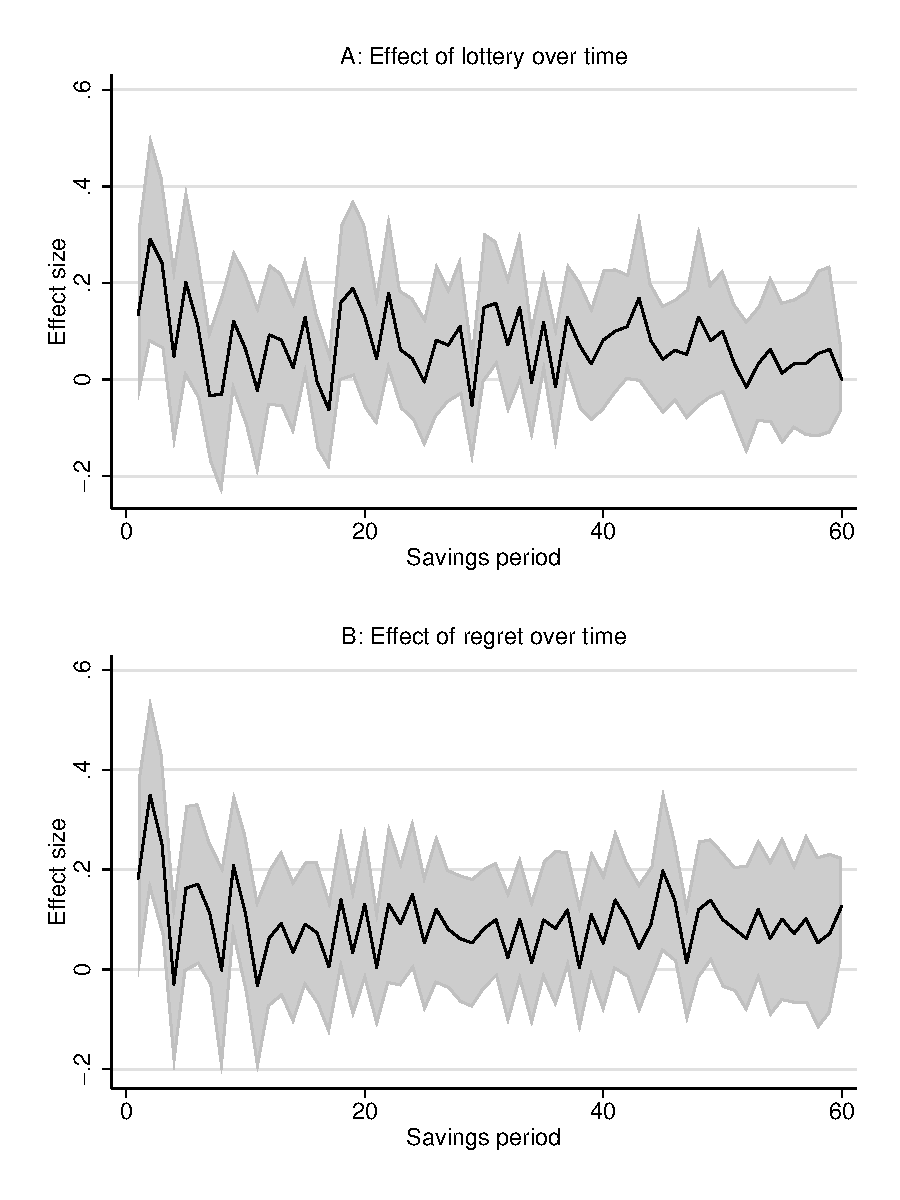
\includegraphics[width=\textwidth]{../../figures/line-timemobile_deposits.pdf}
		% \caption*{\footnotesize \emph{Notes:} Panel A plots the treatment effect of Lottery on number of deposits as a function of savings period. Panel B plots the treatment effect of PLS on number of deposits as a function of savings period. Shaded areas represent period-specific 95\% confidence regions.}
		% \end{figure}

	\subsection{The Effect of PLS on Consumption and Savings by Other Means}

		A related objective of this study is to examine whether PLS act as complements or substitutes to existing savings products. Unsurprisingly, we do not find evidence that PLS crowds out saving by other means since there was no treatment effect on amount saved using PLS. Table \ref{tab:reg-fwersave} reports no statistically significant effect on total saving through M-Pesa or ROSCAs. We do find, however, that respondents in PLS are 14 percentage points ($p < 0.05$) more likely to save with a ROSCA compared to the control group and 16 percentage points ($p < 0.05$) more likely relative to the No Feedback condition. This result is robust to the inclusion of covariates but is significant at the 10\% level when correcting for multiple inference ($p < 0.10$). We find no effect of the No Feedback condition on informal saving. This finding is puzzling but one possible explanation is that participants may be borrowing from ROSCAs in order to fund their PLS deposits. Overall, we do not find that PLS cannibalizes savings from other sources in line with earlier experimental results \parencite{atalay_savings_2014,filiz-ozbay_lottery_2015,dizon_leveraging_2016}.

		\begin{table}[ht]\centering \def\sym#1{\ifmmode^{#1}\else\(^{#1}\)\fi} \caption{Treatment effects -- Savings outside the project} \label{tab:reg-fwersave} \maxsizebox*{\textwidth}{\textheight}{ \begin{threeparttable} \begin{tabular}{l*{5}{c}} \toprule
          &\multicolumn{3}{c}{Effect estimates}&\multicolumn{2}{c}{Sample}\\\cmidrule(lr){2-4}\cmidrule(lr){5-6}
          &\multicolumn{1}{c}{(1)}&\multicolumn{1}{c}{(2)}&\multicolumn{1}{c}{(3)}&\multicolumn{1}{c}{(4)}&\multicolumn{1}{c}{(5)}\\
          &\multicolumn{1}{c}{Lottery}&\multicolumn{1}{c}{Regret}&\multicolumn{1}{c}{\specialcell{Regret-\\Lottery}}&\multicolumn{1}{c}{\specialcell{Control Mean\\(SD)}}&\multicolumn{1}{c}{Obs.}\\
\midrule
Total savings last month&    18.45&   -17.87&   -36.32&    80.31&      284\\
          &  (25.16)&  (14.64)&  (24.06)& (112.74)&         \\
          &   [1.00]&   [1.00]&   [0.20]&         &         \\
M-Pesa savings last month&    -5.42&    -6.71&    -1.29&    20.42&      284\\
          &   (6.34)&   (5.49)&   (5.30)&  (44.67)&         \\
          &   [1.00]&   [1.00]&   [1.00]&         &         \\
ROSCA savings last month&     1.48&     7.37&     5.89&    22.24&      283\\
          &   (6.76)&   (6.79)&   (7.33)&  (42.18)&         \\
          &   [1.00]&   [1.00]&   [0.40]&         &         \\
Saves with a ROSCA&    -0.02&0.14\sym{**}&0.16\sym{**}&     0.54&      284\\
          &   (0.07)&   (0.07)&   (0.07)&   (0.50)&         \\
          &   [1.00]&   [0.40]&[0.00\sym{***}]&         &         \\
\bottomrule \end{tabular} \begin{tablenotes}[flushleft] \footnotesize \item \emph{Notes:} Columns 1--3 report OLS estimates of the treatment effect. Standard errors are in parentheses and FWER adjusted \(p\)-values are in brackets. Observations are at the individual level. * denotes significance at 10 pct., ** at 5 pct., and *** at 1 pct. level. Stars on the coefficient estimates reflect unadjusted \(p\)-values. \end{tablenotes} \end{threeparttable} } \end{table}

% File produced by reg-fwer.do with /Users/justin/Repos/akiba-lottery-pub/data/clean/akiba_wide.dta on 00:15:52 13 Jun 2019 by user justin on Stata 13.1 with seed X27e0a1708256a41cdeaf4038df2ac2a9000400f4

		Table \ref{tab:reg-fwercons} reports effects on how savings from the program was used by participants after it ended. The dependant variables here are dummy variables that indicate whether savings were spent on any of these categories. While we detect some statistically significant effects on airtime and business-related expenditures, these are not significant once adjusting for multiple inference.

		\begin{table}[ht]\centering \def\sym#1{\ifmmode^{#1}\else\(^{#1}\)\fi} \caption{Treatment effects -- Expenditure} \label{tab:reg-fwercons} \maxsizebox*{\textwidth}{\textheight}{ \begin{threeparttable} \begin{tabular}{l*{5}{c}} \toprule
          &\multicolumn{3}{c}{Effect estimates}&\multicolumn{2}{c}{Sample}\\\cmidrule(lr){2-4}\cmidrule(lr){5-6}
          &\multicolumn{1}{c}{(1)}&\multicolumn{1}{c}{(2)}&\multicolumn{1}{c}{(3)}&\multicolumn{1}{c}{(4)}&\multicolumn{1}{c}{(5)}\\
          &\multicolumn{1}{c}{PLS-N}&\multicolumn{1}{c}{PLS-F}&\multicolumn{1}{c}{\specialcell{PLS-F $-$ \\PLS-N}}&\multicolumn{1}{c}{\specialcell{Control Mean\\(SD)}}&\multicolumn{1}{c}{Obs.}\\
\midrule
Airtime   &-0.33\sym{**}&    -0.13&0.20\sym{*}&     0.35&      284\\
          &   (0.15)&   (0.19)&   (0.12)&   (1.47)&         \\
          &   [0.20]&   [1.00]&   [0.40]&         &         \\
Business-related&0.08\sym{*}&0.10\sym{**}&     0.02&     0.06&      284\\
          &   (0.04)&   (0.05)&   (0.05)&   (0.25)&         \\
          &   [0.80]&   [0.20]&   [1.00]&         &         \\
Durable goods&    -0.06&    -0.01&     0.05&     0.13&      284\\
          &   (0.04)&   (0.05)&   (0.04)&   (0.34)&         \\
          &   [0.80]&   [1.00]&   [1.00]&         &         \\
Loan repayment&    -0.01&    -0.02&    -0.01&     0.09&      284\\
          &   (0.04)&   (0.04)&   (0.04)&   (0.28)&         \\
          &   [1.00]&   [1.00]&   [1.00]&         &         \\
Food      &     0.04&    -0.08&-0.12\sym{*}&     0.28&      284\\
          &   (0.07)&   (0.06)&   (0.06)&   (0.45)&         \\
          &   [1.00]&   [1.00]&   [0.40]&         &         \\
Rent and housing payments&    -0.03&    -0.00&     0.03&     0.11&      284\\
          &   (0.04)&   (0.04)&   (0.04)&   (0.31)&         \\
          &   [1.00]&   [1.00]&   [1.00]&         &         \\
Health-related&    -0.02&-0.03\sym{*}&    -0.01&     0.03&      284\\
          &   (0.02)&   (0.02)&   (0.01)&   (0.18)&         \\
          &   [1.00]&   [1.00]&   [1.00]&         &         \\
Other non-durables&     0.01&     0.03&     0.02&     0.01&      284\\
          &   (0.02)&   (0.02)&   (0.03)&   (0.10)&         \\
          &   [1.00]&   [1.00]&   [1.00]&         &         \\
Saved balance&     0.04&     0.06&     0.02&     0.07&      284\\
          &   (0.04)&   (0.04)&   (0.05)&   (0.26)&         \\
          &   [1.00]&   [1.00]&   [1.00]&         &         \\
School-related&     0.08&     0.02&    -0.06&     0.12&      284\\
          &   (0.05)&   (0.05)&   (0.05)&   (0.32)&         \\
          &   [0.80]&   [1.00]&   [1.00]&         &         \\
Transfers &     0.02&    -0.00&    -0.02&     0.02&      284\\
          &   (0.03)&   (0.02)&   (0.03)&   (0.15)&         \\
          &   [1.00]&   [1.00]&   [1.00]&         &         \\
Travel    &    -0.00&    -0.00&     0.00&     0.02&      284\\
          &   (0.02)&   (0.02)&   (0.02)&   (0.15)&         \\
          &   [1.00]&   [1.00]&   [1.00]&         &         \\
Did not save&    -0.02&    -0.01&     0.01&     0.10&      284\\
          &   (0.04)&   (0.04)&   (0.04)&   (0.30)&         \\
          &   [1.00]&   [1.00]&   [1.00]&         &         \\
\bottomrule \end{tabular} \begin{tablenotes}[flushleft] \footnotesize \item \emph{Notes:} Columns 1--3 report OLS estimates of the treatment effect. Standard errors are in parentheses and FWER adjusted \(p\)-values are in brackets. Observations are at the individual level. * denotes significance at 10 pct., ** at 5 pct., and *** at 1 pct. level. Stars on the coefficient estimates reflect unadjusted \(p\)-values. \end{tablenotes} \end{threeparttable} } \end{table}

% File produced by reg-fwer.do with /Users/justin/Repos/akiba-lottery-pub/data/clean/akiba_wide.dta on 11:51:58 25 Oct 2020 by user justin on Stata 13.1 with seed X27e0a1708256a41cdeaf4038df2ac2a9000400f4

	\subsection{PLS Increases Self-Reported Gambling}

		At the end of the trial, we asked participants whether they gambled more or less than they usually do apart from participating in the savings program. We estimate a multinomial logit regression to examine how treatment affects responses. As reported in Table \ref{tab:reg-mlogfreq}, we find that the risk of gambling more relative to no change is increased by a factor of 3.03 for participants in the PLS group compared to control ($p < 0.01$). The relative risk of gambling more also increases by a factor of 1.87 for PLS with feedback compared to without feedback. We find no average effects for participants using PLS without feedback. Examining participant input at the end of the experiment provides some evidence as to why PLS might encourage gambling. Table \ref{tab:reg-fwerself} reports that PLS users in either feedback condition feel they are more lucky compared to participants in the control group by almost 5 std. deviations\footnote{This outcome was measured on a scale from 1-3 with 3 being the most lucky. Scales are standardized to mean zero and std. dev. 1 when used as outcomes in regressions.} (PLS: $\hat \beta = 4.97, p < 0.01$; No Feedback: $\hat \beta = 4.77, p < 0.01$). It is plausible that winning money from the lottery may have altered individuals' perception of their chances of winning at large. Table \ref{tab:het-gam_mediancpgi_z_0} shows no heterogeneity of this effect by a baseline measure of problem gambling.

		\textcite{atalay_savings_2014} and \textcite{dizon_leveraging_2016} both observe large reductions in gambing expenditure in order to finance savings with PLS. It is possible that while PLS is a substitute for gambling with a cash windfall (as in their study), it interacts differently when indviduals already have a history of gambling. \textcite{cookson_when_2016} offered individuals in Nebraska access to an PLS and observed cash withdrawals at casinos as a measure of gambling behavior. They find reductions in transactions between 7-15\% and credit the effect to substition of casino gambling with PLS. Our measure for gambling activity, as a self-report, is likely susceptible to experimenter demand and it is unclear in what direction this might bias our estimate. With this caveat in mind, the effect provides some experimental evidence of a complementary relationship between PLS and broader gambling behavior.

		\begin{table}[h]\centering \def\sym#1{\ifmmode^{#1}\else\(^{#1}\)\fi} \caption{Multinomial treatment effects -- Gambling behavior} \label{tab:reg-mlogfreq} \maxsizebox*{\textwidth}{\textheight}{ \begin{threeparttable} \begin{tabular}{l*{5}{c}} \toprule
          &\multicolumn{4}{c}{Relative risk ratio}&\multicolumn{1}{c}{Sample}\\\cmidrule(lr){2-5}\cmidrule(lr){6-6}
          &\multicolumn{1}{c}{(1)}&\multicolumn{1}{c}{(2)}&\multicolumn{1}{c}{(3)}&\multicolumn{1}{c}{(4)}&\multicolumn{1}{c}{(5)}\\
          &\multicolumn{1}{c}{Constant}&\multicolumn{1}{c}{No Feedback}&\multicolumn{1}{c}{PLS}&\multicolumn{1}{c}{\specialcell{PLS-\\No Feedback}}&\multicolumn{1}{c}{Obs.}\\
\midrule
Gambled less&     0.22&     0.91&     1.69&     1.86&      284\\
          &   (0.06)&   (0.38)&   (0.66)&   (0.76)&         \\
Gambled more&     0.16&     1.62&     3.03&     1.87&      284\\
          &   (0.05)&   (0.69)&   (1.23)&   (0.69)&         \\
\bottomrule \end{tabular} \begin{tablenotes}[flushleft] \footnotesize \item \emph{Notes:} This table reports estimates from a multinomial logit regression of the categorial response on treatment assigment. Each row corresponds to a response category with the baseline value as . Column 1 reports the constant term corresponding to the mean of the control group. Columns 2--3 reports the treatment effect in relative risk ratios compared to the control group. Column 4 reports the difference between the two PLS treatments. Standard errors are in parentheses. Column 5 reports the number of observations in the analytic sample. Observations are at the individual level. \end{tablenotes} \end{threeparttable} } \end{table}

% File produced by reg-mlogit.do with /Users/justin/Repos/akiba-lottery-pub/data/clean/akiba_wide.dta on 19:20:14 12 Aug 2020 by user justin on Stata 13.1 with seed X71d1d353b37e281e006fa26738e26f4500044a1c

		\begin{table}[ht]\centering \def\sym#1{\ifmmode^{#1}\else\(^{#1}\)\fi} \caption{Treatment effects -- Self-perceptions} \label{tab:reg-fwerself} \maxsizebox*{\textwidth}{\textheight}{ \begin{threeparttable} \begin{tabular}{l*{5}{c}} \toprule
          &\multicolumn{3}{c}{Effect estimates}&\multicolumn{2}{c}{Sample}\\\cmidrule(lr){2-4}\cmidrule(lr){5-6}
          &\multicolumn{1}{c}{(1)}&\multicolumn{1}{c}{(2)}&\multicolumn{1}{c}{(3)}&\multicolumn{1}{c}{(4)}&\multicolumn{1}{c}{(5)}\\
          &\multicolumn{1}{c}{PLS-N}&\multicolumn{1}{c}{PLS-F}&\multicolumn{1}{c}{\specialcell{PLS-F $-$ \\PLS-N}}&\multicolumn{1}{c}{\specialcell{Control Mean\\(SD)}}&\multicolumn{1}{c}{Obs.}\\
\midrule
Do you see yourself as a saver?&    -0.20&    -0.09&     0.11&    -0.00&      284\\
          &   (0.15)&   (0.14)&   (0.15)&   (1.00)&         \\
          &   [0.60]&   [1.00]&   [1.00]&         &         \\
Are you in general a lucky person?&4.77\sym{***}&4.97\sym{***}&     0.20&    -0.00&      284\\
          &   (0.20)&   (0.18)&   (0.23)&   (1.00)&         \\
          &[0.00\sym{***}]&[0.00\sym{***}]&   [0.80]&         &         \\
Do you feel you saved enough?&     0.19&    -0.09&-0.28\sym{*}&     0.00&      284\\
          &   (0.15)&   (0.15)&   (0.15)&   (1.00)&         \\
          &   [0.60]&   [1.00]&   [0.20]&         &         \\
How did you feel not saving?&    -0.02&     0.06&     0.08&    -0.00&      284\\
          &   (0.16)&   (0.15)&   (0.16)&   (1.00)&         \\
          &   [1.00]&   [1.00]&   [1.00]&         &         \\
\bottomrule \end{tabular} \begin{tablenotes}[flushleft] \footnotesize \item \emph{Notes:} Columns 1--3 report OLS estimates of the treatment effect. Standard errors are in parentheses and FWER adjusted \(p\)-values are in brackets. Observations are at the individual level. * denotes significance at 10 pct., ** at 5 pct., and *** at 1 pct. level. Stars on the coefficient estimates reflect unadjusted \(p\)-values. \end{tablenotes} \end{threeparttable} } \end{table}

% File produced by reg-fwer.do with /Users/justin/Repos/akiba-lottery-pub/data/clean/akiba_wide.dta on 11:52:03 25 Oct 2020 by user justin on Stata 13.1 with seed X27e0a1708256a41cdeaf4038df2ac2a9000400f4

\section{Conclusion} \label{sec:conclusion}

	There is an abundance of evidence on the promise of product design in encouraging savings among the poor. We conducted a randomized experiment testing a prize-linked savings product with informal residents in Nairobi, Kenya. Utilizing a mobile savings platform, we randomly assign respondents to a savings account with a certain, matching incentive, a lottery incentive, and a lottery incentive with feedback on ex post potential lottery winnings. We set the fixed match of 5\% equivalent in expectation to the lottery prize so that comparing the two groups identifies the effect of stochastic incentives compared to deterministic incentives. After observing account transactions over a 60-day savings period, we find that participants in the PLS group made between 5-6 more deposit transactions than the matched payments group without a corresponding increase in amount saved. We further find no effects on amounts saved through other channels except that participants assigned to the PLS treatment with feedback were 14 percentage points more likely to have saved with a ROSCA. Finally, treated participants are 15 percentage points more likely than the control group to report that they gamble more.

	Comparing the two PLS treatments provides a test of regret aversion as an underlying mechanism behind the increased usage that we observe. Under this hypothesis, marginal savers will be induced to make deposits in order to minimize the anticipated regret from missing out on the prize. Our findings are consistent with regret minimization: individuals make 20\% more deposits when they expect to be given feedback about lottery results regardless of their decision to save. Participants in the feedback condition are also 8\% more likely to make a deposit as a result of having recently won a lottery without a prize. Our interpretation for this result is that recently experienced regret may intensify aversion to anticipated regret and further motivate deposits. Overall, we document important differences between PLS and fixed-incentive schemes when it comes to encouraging savings and show that theories of regret aversion hold sway in the design of savings products.

	The welfare implications of our results are far from evident, especially since regret aversion, as a non-standard model of choice, complicates conventional normative approaches\footnote{We direct readers to \textcite{bernheim_behavioral_2009} for a discussion of recent behavioral approaches to welfare.}. Nevertheless, our findings show that lottery-like incentives, particularly those provide feedback on their outcomes, can be used by policymakers to influence financial decisions. Since PLS motivates deposits through the presence of a lottery, it could prove to be more cost-effective than a fixed subsidy of an equivalent, expected size.

	% on welfare: sarver and gee provide argument about why PLS could be welfare decreasing

	If PLS increases deposits but are ineffective at increasing the savings rate, can they still useful from a development perspective? Two recent field experiments suggest so. \textcite{schaner_persistent_2018} finds moderate short run effects of interest rate subsidies on savings but documents impressive effects on income and capital stock over two years after the incentive expired. They argue that the temporary incentives accomplished increased long run account usage through habit formation. \textcite{gertler_long-term_2017} observes initially lower account balances among individuals who opened PLS accounts compared to control, but the 41\% additional open accounts induced by PLS continued to be used in the long run and maintained balances comparable to the control group. If PLS opens the door for greater account usage in the short run (as we report in this study), then it could lead to persistent changes in financial decisionmaking over time.

	The prevalance of gambling may also be a policy outcome of interest in its own right. While there is evidence from both the lab and the field that PLS displaces other forms of gambling as its substitute, we provide limited evidence that individuals with PLS accounts gamble relatively more than the control group. PLS may also be disadvantageous from this perspective if it merely represents another consumption opportunity for gambling and not as a vehicle to accumulate savings.

	Our study design is limited in that we could not observe participants' entire portfolio of financial decision over the trial period. That type of data could allow us to understand, for example, how lottery plays were being financed, how PLS affected the effective savings rate over time, and whether PLS changed participants' pattern of daily consumption. Moreover, the data could be used for structural estimation of behavioral parameters (as in \textcite{filiz-ozbay_lottery_2015}) in a mdoel of regret aversion. As discussed previously, a long-term examination of outcomes is promising and could have material consequences for welfare. Taking a longer perspective could also prove useful in the study of regret aversion over repeated settings, an area of research still at the frontier of the behavioral literature.

	\clearpage

\newpage

\printbibliography

\newpage

\appendix

\section{A Simple Model of Saving with PLS} \label{sec:model}

	In this section, we formalize the intuition behind how feedback on lottery results works to increase the number of deposits to PLS accounts. We present a simple model of an individual facing a one-shot, binary decision to save or not save with PLS with and without feedback.

	% need to argue that even with a discount factor the results hold qualitatively. we should see that more patient people will have a greater effect

	% why binary and not continuous? can use it to show effects on the exensive margin not intensive

	Regret-sensitive preferences are defined as follows. Let $f, g \in B$ be prospects in the individual's choice set. $i$ indexes the events in a finite, discrete state space. An individual who chooses $f$ when event $i$ occurs evaluates outcomes according to a bivariate utility function.\footnote{The theoretical literature does not typically make such a restrictive functional form assumption but we do so here for expositional purposes.}

		\[ Q(f_i; g_i) \equiv u(f_i) + \gamma R(u(f_i) - u(g_i)) \]

	$f_i$ is the return on the deposit when event $i$ occurs, $u$ is a von Neumann-Morgenstern utility function, and $R$ is a regret function that evaluates utility differences between outcomes from the selected lottery to outcomes from the foregone lottery, state-by-state. $\gamma \geq 0$ is a parameter that governs the degree of regret/rejoicing.

	Define $\Psi(f_i; g_i) \equiv Q(f_i; g_i) - Q(g_i; f_i)$ as the advantage, in utility terms, of obtaining $f_i$ over $g_i$ . Regret theory holds if there exists a continuous, strictly increasing function $u$ and a continuous, strictly increasing, and skew-symmetric function $\Psi$ such that

		\[ f \succsim g \leftrightarrow \sum_{i} p_{i} \cdot \Psi (f_i; g_i) \geq 0 \]

	\noindent where $p_i$ is the probability of an event $i$. Skew-symmetry implies $R(0) = 0$ and means that no regret/rejoicing is experienced when outcomes are identical. The convexity of $\Psi$ over gains corresponds to regret aversion. When $\Psi$ is linear ($\gamma = 0$ in this parameterization), the individual behaves as if she were maximizing expected utility.

	When an individual in the PLS treatment makes a deposit, her payoff $y$ is proportional to a match rate applied to the deposit. The rate (and payoff) is determined by a lottery $\ell = (y_i, p_i)_{i=1}^{4}$ defined over the event of no matches, one match, two matches, and four matches of a sequence of numbers in a lottery ticket to a randomly generated sequence. When she chooses not to make a deposit, the individual obtains zero returns with certainty.

	How does feedback regarding the resolution of the lottery affect anticipated regret? We postulate that when the decisionmaker makes a choice that obscures the resolution of the lottery that she is unable to make comparisons to foregone outcomes. In our model, a decision that results in no feedback is associated with an expected utility over final outcomes of $\sum_{i} p_{i} \cdot u(f_i)$.\footnote{Original theories of regret \parencite{loomes_regret_1982,bell_risk_1983} do not explicitly model the role of feedback on decisions. In light of empirical evidence, some applications disallow the calculation of the regret term when foregone lotteries remain unresolved as we do here \parencite{strack_too_2019,filiz-ozbay_auctions_2007} while others impose a less extreme assumption that regret/rejoicing is less intense withou feedback \parencite{somasundaram_regret_2017,humphrey_feedback-conditional_2004}.}

	The expected utility associated with choosing to save with PLS in both the feedback and no feedback treatments is equivalent since saving will result in the resolution of the lottery in both conditions.

		\[ \sum_{i=1}^{4} p_i \cdot \left [ u(y_i) + \gamma R(u(y_i) - u(0)) \right ] \]

	The expected utility associated with not saving with feedback is

		\[ u(0) + \sum_{i=1}^{4} p_i \cdot \gamma R(u(0)-u(y_i)) \]

	\noindent but not saving without feedback attains the decisionmaker $u(0)$. Note that since there is no possibility of negative returns in the lottery, $R(u(0) - u(y_i)) \leq 0$ for all $i$. As a result, the expected utility from not saving with feedback is weakly less than the utility from not saving with feedback.

	\[ \sum_{i} p_{i} \cdot \Psi_\text{PLS} (y_i; 0)  \geq \sum_{i} p_{i} \cdot \Psi_\text{NF} (y_i; 0) \]

	The relationship is a strict inequality if $\gamma > 0$: the individual exhibits some degree of regret aversion. This expression encapsulates our hypothesis that with regret aversion, marginal decisionmakers is more likely to make a deposit under PLS with feedback than PLS where feedback is conditional on saving.

	% maybe define theorems and propositions

	% additional results on the relationship between regret, risk, and discounting (but no het effects)

	\clearpage

\section{Heterogeneous Treatment Effects}
	
	\begin{table}[ht]\centering \def\sym#1{\ifmmode^{#1}\else\(^{#1}\)\fi} \caption{Heterogeneous effects -- Primary outcomes by currently saves} \label{tab:het-save_dosave_0} \maxsizebox*{\textwidth}{\textheight}{ \begin{threeparttable} \begin{tabular}{l*{4}{c}} \toprule
                &\multicolumn{1}{c}{(1)}&\multicolumn{1}{c}{(2)}&\multicolumn{1}{c}{(3)}&\multicolumn{1}{c}{(4)}\\
                &\multicolumn{1}{c}{Total no. of deposits}&\multicolumn{1}{c}{Total deposit amount}&\multicolumn{1}{c}{Saves with a ROSCA}&\multicolumn{1}{c}{Gamble more}\\
\midrule
No Feedback     &     8.07\sym{**} &     2.05         &    -0.00         &     0.06         \\
                &   (4.07)         &   (4.49)         &   (0.11)         &   (0.07)         \\
No Feedback $\times$ \\ Currently saves&    -6.16         &    -5.25         &    -0.03         &    -0.00         \\
                &   (5.23)         &   (6.57)         &   (0.15)         &   (0.10)         \\
PLS             &     8.26\sym{**} &     3.42         &     0.24\sym{**} &     0.18\sym{**} \\
                &   (3.23)         &   (3.77)         &   (0.10)         &   (0.07)         \\
PLS $\times$ \\ Currently saves&    -4.32         &    -9.25         &    -0.19         &    -0.06         \\
                &   (4.87)         &   (5.64)         &   (0.14)         &   (0.11)         \\
Currently saves &     5.62\sym{**} &     7.44         &     0.14         &     0.09         \\
                &   (2.82)         &   (4.56)         &   (0.10)         &   (0.06)         \\
Constant        &    10.50\sym{***}&    10.69\sym{***}&     0.47\sym{***}&     0.07\sym{*}  \\
                &   (1.79)         &   (2.73)         &   (0.08)         &   (0.04)         \\
\midrule
Adjusted \(R^{2}\)&    0.009         &   -0.004         &    0.015         &    0.015         \\
Control mean    &    13.66         &    14.87         &     0.54         &     0.12         \\
No Feedback \emph{p}-value&     0.56         &     0.51         &     0.71         &     0.45         \\
PLS \emph{p}-value&     0.28         &     0.17         &     0.60         &     0.15         \\
Observations    &      311         &      311         &      284         &      284         \\
\bottomrule \end{tabular} \begin{tablenotes}[flushleft] \footnotesize \item \emph{Notes:} This table reports OLS estimates of the treatment effect and its interaction with baseline. Standard errors are in parentheses. * denotes significance at 10 pct., ** at 5 pct., and *** at 1 pct. level. We also report the \(p\)-values for joint tests on the direct treatment effect conditional on the baseline covariate $= 1$. \end{tablenotes} \end{threeparttable} } \end{table}

% File produced by akiba_estimate.do with /Users/justin/Repos/akiba-lottery-pub/data/clean/akiba_wide.dta on 11:37:00 19 Mar 2020 by user justin on Stata 13.1 with seed X440b457b8aac484a7d965296a0f1c153000412ab
	\begin{table}[htbp]\centering \def\sym#1{\ifmmode^{#1}\else\(^{#1}\)\fi} \caption{Heterogeneous effects - Primary outcomes by risk averse} \label{tab:het-pref_riskaverse_0} \maxsizebox*{\paperwidth}{\paperheight}{ \begin{threeparttable} \begin{tabular}{l*{4}{c}} \toprule
                &\multicolumn{1}{c}{(1)}&\multicolumn{1}{c}{(2)}&\multicolumn{1}{c}{(3)}&\multicolumn{1}{c}{(4)}\\
                &\multicolumn{1}{c}{Total no. of deposits}&\multicolumn{1}{c}{Daily avg. no. of deposits}&\multicolumn{1}{c}{No. of days saved}&\multicolumn{1}{c}{Gamble more}\\
\midrule
Lottery         &     7.87\sym{**} &    -0.09         &     6.65\sym{**} &     0.08         \\
                &   (3.63)         &   (0.07)         &   (2.78)         &   (0.08)         \\
Lottery $\times$ \\ Risk averse&    -7.63         &     0.13         &    -6.23         &    -0.05         \\
                &   (4.92)         &   (0.08)         &   (4.10)         &   (0.10)         \\
Regret          &     7.83\sym{**} &    -0.06         &     7.01\sym{**} &     0.15\sym{*}  \\
                &   (3.50)         &   (0.06)         &   (2.92)         &   (0.08)         \\
Regret $\times$ \\ Risk averse&    -4.62         &     0.10         &    -4.50         &    -0.01         \\
                &   (4.89)         &   (0.07)         &   (4.17)         &   (0.11)         \\
Risk averse     &     0.50         &    -0.12\sym{**} &     1.18         &    -0.05         \\
                &   (2.97)         &   (0.06)         &   (2.55)         &   (0.07)         \\
Constant        &    13.42\sym{***}&     1.22\sym{***}&    11.22\sym{***}&     0.14\sym{***}\\
                &   (1.99)         &   (0.06)         &   (1.63)         &   (0.05)         \\
\midrule
Adjusted \(R^{2}\)&    0.017         &    0.004         &    0.015         &    0.015         \\
Control mean    &    13.66         &     1.16         &    11.78         &     0.12         \\
Lottery \emph{p}-value&     0.94         &     0.36         &     0.89         &     0.65         \\
Regret \emph{p}-value&     0.35         &     0.38         &     0.40         &     0.07         \\
Observations    &      311         &      275         &      311         &      284         \\
\bottomrule \end{tabular} \begin{tablenotes}[flushleft] \footnotesize \item \emph{Notes:} This table reports OLS estimates of the treatment effect and its interaction with baseline. Standard errors are in parentheses. * denotes significance at 10 pct., ** at 5 pct., and *** at 1 pct. level. We also report the \(p\)-values for joint tests on the direct treatment effect conditional on the baseline covariate $= 1$. \end{tablenotes} \end{threeparttable} } \end{table}

% File produced by akiba_estimate.do with /Users/Justin/Repos/akiba-lottery-pub/data/clean/akiba_wide.dta on 14:36:15  6 Mar 2017 by user Justin on Stata 13.1 with seed Xab009a28c79e3115499f664c1f29957300040c93
	\begin{table}[ht]\centering \def\sym#1{\ifmmode^{#1}\else\(^{#1}\)\fi} \caption{Heterogeneous effects -- Primary outcomes by above median i. point} \label{tab:het-pref_medianindiff_0} \maxsizebox*{\textwidth}{\textheight}{ \begin{threeparttable} \begin{tabular}{l*{4}{c}} \toprule
                &\multicolumn{1}{c}{(1)}&\multicolumn{1}{c}{(2)}&\multicolumn{1}{c}{(3)}&\multicolumn{1}{c}{(4)}\\
                &\multicolumn{1}{c}{Total no. of deposits}&\multicolumn{1}{c}{Total deposit amount}&\multicolumn{1}{c}{Saves with a ROSCA}&\multicolumn{1}{c}{Gamble more}\\
\midrule
Lottery         &     3.06         &    -8.41         &     0.02         &     0.08         \\
                &   (3.10)         &   (5.14)         &   (0.10)         &   (0.07)         \\
Lottery $\times$ \\ Above median i. point&     3.71         &    16.03\sym{**} &    -0.07         &    -0.03         \\
                &   (5.23)         &   (6.95)         &   (0.15)         &   (0.10)         \\
Regret          &     9.75\sym{***}&    -4.02         &     0.24\sym{**} &     0.19\sym{**} \\
                &   (3.47)         &   (5.07)         &   (0.10)         &   (0.08)         \\
Regret $\times$ \\ Above median i. point&    -7.98         &     4.62         &    -0.20         &    -0.09         \\
                &   (4.88)         &   (5.88)         &   (0.14)         &   (0.11)         \\
Above median i. point&     0.63         &    -8.85\sym{*}  &     0.08         &     0.02         \\
                &   (2.95)         &   (4.82)         &   (0.10)         &   (0.07)         \\
Constant        &    13.33\sym{***}&    19.42\sym{***}&     0.50\sym{***}&     0.11\sym{**} \\
                &   (1.97)         &   (4.51)         &   (0.07)         &   (0.05)         \\
\midrule
Adjusted \(R^{2}\)&    0.018         &    0.010         &    0.011         &    0.010         \\
Control mean    &    13.66         &    14.87         &     0.54         &     0.12         \\
Lottery \emph{p}-value&     0.11         &     0.10         &     0.66         &     0.55         \\
Regret \emph{p}-value&     0.61         &     0.84         &     0.70         &     0.22         \\
Observations    &      311         &      311         &      284         &      284         \\
\bottomrule \end{tabular} \begin{tablenotes}[flushleft] \footnotesize \item \emph{Notes:} This table reports OLS estimates of the treatment effect and its interaction with baseline. Standard errors are in parentheses. * denotes significance at 10 pct., ** at 5 pct., and *** at 1 pct. level. We also report the \(p\)-values for joint tests on the direct treatment effect conditional on the baseline covariate $= 1$. \end{tablenotes} \end{threeparttable} } \end{table}

% File produced by akiba_estimate.do with /n/homeserver2/user2a/justinra/repos/akiba-lottery-pub/data/clean/akiba_wide.dta on 07:12:01 21 Feb 2018 by user justinra on Stata 13.1 with seed X148d7873983cbab146cfd6c3f6771e1900043266
	\begin{table}[ht]\centering \def\sym#1{\ifmmode^{#1}\else\(^{#1}\)\fi} \caption{Heterogeneous effects -- Primary outcomes by above median cpgi} \label{tab:het-gam_mediancpgi_z_0} \maxsizebox*{\textwidth}{\textheight}{ \begin{threeparttable} \begin{tabular}{l*{4}{c}} \toprule
                &\multicolumn{1}{c}{(1)}&\multicolumn{1}{c}{(2)}&\multicolumn{1}{c}{(3)}&\multicolumn{1}{c}{(4)}\\
                &\multicolumn{1}{c}{Total no. of deposits}&\multicolumn{1}{c}{Total deposit amount}&\multicolumn{1}{c}{Saves with a ROSCA}&\multicolumn{1}{c}{Gamble more}\\
\midrule
Lottery         &     2.53         &    -1.40         &    -0.09         &    -0.01         \\
                &   (3.29)         &   (3.45)         &   (0.10)         &   (0.07)         \\
Lottery $\times$ \\ Above median CPGI&     4.38         &     1.69         &     0.16         &     0.16         \\
                &   (5.22)         &   (7.00)         &   (0.15)         &   (0.11)         \\
Regret          &     6.17\sym{*}  &     0.79         &     0.13         &     0.11         \\
                &   (3.59)         &   (3.44)         &   (0.10)         &   (0.08)         \\
Regret $\times$ \\ Above median CPGI&    -1.79         &    -5.46         &     0.03         &     0.07         \\
                &   (4.79)         &   (5.89)         &   (0.14)         &   (0.12)         \\
Above median CPGI&    -2.88         &     2.49         &     0.00         &    -0.06         \\
                &   (2.93)         &   (4.86)         &   (0.10)         &   (0.07)         \\
Constant        &    15.06\sym{***}&    13.66\sym{***}&     0.54\sym{***}&     0.15\sym{***}\\
                &   (2.27)         &   (2.55)         &   (0.07)         &   (0.05)         \\
\midrule
Adjusted \(R^{2}\)&    0.009         &   -0.010         &    0.013         &    0.014         \\
Control mean    &    13.66         &    14.87         &     0.54         &     0.12         \\
Lottery \emph{p}-value&     0.09         &     0.96         &     0.48         &     0.06         \\
Regret \emph{p}-value&     0.17         &     0.33         &     0.13         &     0.03         \\
Observations    &      311         &      311         &      284         &      284         \\
\bottomrule \end{tabular} \begin{tablenotes}[flushleft] \footnotesize \item \emph{Notes:} This table reports OLS estimates of the treatment effect and its interaction with baseline. Standard errors are in parentheses. * denotes significance at 10 pct., ** at 5 pct., and *** at 1 pct. level. We also report the \(p\)-values for joint tests on the direct treatment effect conditional on the baseline covariate $= 1$. \end{tablenotes} \end{threeparttable} } \end{table}

% File produced by akiba_estimate.do with /Users/justin/Repos/akiba-lottery-pub/data/clean/akiba_wide.dta on 10:05:12 14 Jun 2019 by user justin on Stata 13.1 with seed X32b3301a224bcb612cd99bbd84ad23ad0004026c

	\clearpage

\end{document}

% Student feedback

% Exposition on regret aversion

% x	It is good to see the result is consistent with regret aversion? Are there other plausible explanations? 

% x	Does regret aversion explain why low-income individuals are more likely to play the lottery in general?

% x	Interesting to see the paper tying behavioral theory in RCT. Maybe you could spend a little more time on the intuition of the theory though to help understand the empirical results.

% Interpretation of results 

% x	I'm not sure what the regret theory portion adds. Probably worth just presenting the intuition for our purposes. Also my evergreen recommendation of doing more explicit functional form modeling / structural stuff (especially with the regret function), even though the assumptions might be strong. I'm not sure why the timing of deposits point is compelling; why wouldn't it show up without regret aversion? (I'm also angry about one * for 10% significance but ¯\_(ツ)_/¯. Slide 23's caption seems to have the baseline value as blank. (You could also make this slide a graph.)

% Framing of paper

% x	For me this paper is more about verifying the regret aversion rather than facilitating savings, but you were motivating the audience with more emphasis given to the savings story. 

% x	I would emphasize that more while perhaps highlighting anecdotes or other studies that help further motivate the kind of behavior that you're seeing.

% x	I think the framing works well (disagreeing with comment made in presentation) - it is important to note interventions with small/no effects on savings. 

% Additional analyses

% 	Can your pre-treatment measures of risk aversion etc push back against the notion that this is people paying to gamble for a couples months? If gamblers are more risk-loving, then you could look for heterogeneity on this measure.

% 	This was a very interesting experiment. I'm wondering whether it's possible for you to distinguish between regret aversion and disappointment aversion as a factor that induces the difference between treatment behaviors. In regret aversion, you experience disutility from not having made a better choice, given state; in disappointment aversion, the disutility comes from the state itself not being better, given your choice. It's essentially a "I could have done better" mindset vs "Things could have been better for me" mindset. Is it possible to distinguish between these two in your experiment? If yes, that could provide additional behavioral findings for your results.

% 	I think this experiment on regret is really interesting. The design of using feedback is a very smart and intuitive way. I was wondering if there is way to quantify this regret aversion by combing the experimental data and the regret theory. Maybe by different profiles of the lottery?

% 	I think this might be out of scope, I am just curious about patterns of saving in PLS groups. (with and without feedback) Isn't is that people would save more right before the withdrawal days (30th day and final day) because cost of saving for doing lottery is lower? If people with feedback already use money to do lottery long before withdrawal days, then would people without feedback (might not spend money to save compared to ones with feedback) use more money to do lottery right before the withdrawal days? If this is true, then PLS with  feedback could make people to save more uniformly during the period, which could help them to smooth their consumption and get insurance against adverse events? Sorry for lacking of rigorous logic on this but it is just my curiosity.

% Policy/welfare discussion

% 	I liked it. I only wonder it's external validity. I'm just not sure if the behaviors in developing countries is same as that for developed countries.

% 	Maybe emphasize the null effect on savings early on. Also, is there any reason why the frequency of deposits is an important margin to look at? Perhaps to reduce the poverty tax on money holdings, e.g., being forced to lend money to family members?

% 	Pretty good! One thing that would be nice to see is the distribution of the interest rate lottery--if you get an expected interest rate of 5\% by having some low probability high/low interest rate outcomes, this would be useful to see. It is also interesting that you find an increase in savings usage, but no real change in amount saved/interest earned. Given that, I would probably talk less about the welfare/policy value of these PLS accounts (politicians can maybe point to higher savings usage as success, but I do not think that increased savings usage a priori socially beneficial, especially when the savings amount does not change) unless you can really sell this habit formation point you mentioned at the very end. Perhaps you could do a habit-formation study as a followup?

% 	The role of regret in prize-linked savings: I find it interesting that PLS can be complementary to the gambling. Can we think that PLS makes people have more interest in gambling behavior through lottery participation, and therefore the likelihood of gambling increases? From the perspective of government or policymakers, they may be reluctant to use this policy to prevent citizens' gambling behavior.

% 	This is a question on framing: if this paper aims to provide policy implications, then it might be beneficial to add more discussions on what are some potential obstacles bigger institutions (NGOs for example) may face when they want to launch such saving programs. I guess you discuss in the full paper, but it would be interesting to discuss how important the distribution of the curvature of the utility function (regarding regret) tell us whether such products should exist (trade-off between profit and specific welfare weight for poor people’s savings) 